%************************************************
\chapter{Theoretical Background }
\label{ch:theory} % $\mathbb{ZNR}$
%************************************************

%And is it over now, do you know how
%Pickup the pieces and go home.
%Fleetwood Mac, \textit{Rumours}, 1977
%Press your space face close to mine, love
%\begin{flushright}{\slshape    
%	I think, I'm looking on the dark side \\
%	But everyday you hurt my pride \\
%	I'm over my head \\
%	Oh, but it sure feels nice} \\ \medskip
%    --- {Fleetwood Mac, \textit{Over My Head}, 1975}
%\end{flushright}

\section{A Brief History of Dark Matter}
Our understanding of the universe develops in a leap-frog of theory and observation, one catching up to and surpassing the other as technology improves, to be passed in turn by a new idea or new observation. The picture of dark matter commonly accepted today is much different than what Zwicky anticipated in 1933 when he found that the velocity dispersion of the galaxies in the Coma Cluster was much larger than expected from the Virial Theorem \cite{Zwicky1933}. This observation is typically cited as popularizing the term ``dark matter'', and starting the hunt for the mysterious invisible substance. Zwicky postulated that the faster rotation was caused by dark matter consisting of cold gas or stars and both macro- and micro-scopic solid bodies, and estimated that there was about 400 times more dark matter than visible matter. Smith, a contemporary of Zwicky's, did a similar analysis with the Virgo Cluster and his results yielded a much smaller dark matter to visible matter ratio \cite{Bertone2016}. Meanwhile, many in the astrophysics community disagreed with an underlying assumption of these analyses and argued that galaxy clusters are not at equilibrium so the Virial Theorem does not apply \cite{Bertone2016}. At the time, the only consensus reached was that more information was needed to understand the dynamics of galaxy clusters. 

In the 1970's, a new technology called the image tube spectrograph allowed Vera Rubin and Kent Ford, the developer of the spectrograph, to measure the rotational velocity of the Andromeda Galaxy at different points along its radius (called a galactic rotation curve) \cite{Rubin1970}. The new data were of higher quality than previous attempts at measuring galactic rotation curves, and the result, that the galaxy was rotating faster than expected at large radius, indicating ``hidden mass,'' was soon replicated by others \cite{Bertone2016}. Over the next decade, a significant number of galactic rotation curves were obtained, all showing essentially the same result: galaxies were rotating faster than expected at high radii, indicating that the masses of galaxies continued to grow past where their lights dimmed. A figure showing this characteristic behavior in 21 galaxies from a 1980 review paper \cite{Rubin1980} is shown in Figure~\ref{fig:curves}. Another argument in favor of dark matter came from contemporary numerical simulations of galactic gravitational dynamics. At first, many simulations showed that disk galaxies were unstable, in contradiction with many observations \cite{Bertone2016}. However, Ostriker and Peebles demonstrated that if the galactic disk was embedded in a massive (i.e. gravitationally interactive) spherical halo, the disk was stable \cite{Peebles1973}.

\begin{figure}[htbp]
\begin{center}
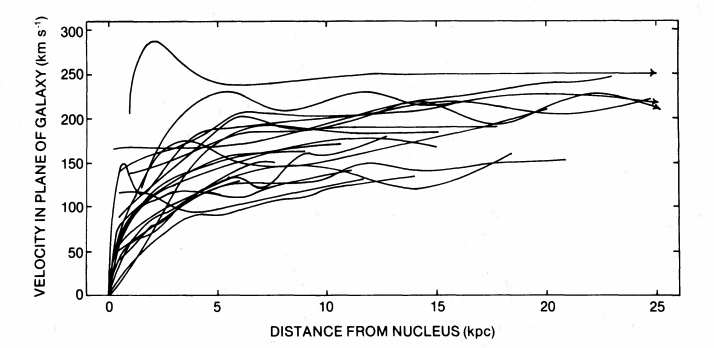
\includegraphics[width=\textwidth]{figures/theory/rot_curves.png}
\caption{Superposition of 21 rotation curves from galaxies with a large range of radii and luminosities. All of these galaxies have a distinctive flat rotation curve at large radii. Figure from \cite{Rubin1980}.}
\label{fig:curves}
\end{center}
\end{figure}


In order to explain the behavior of galactic rotation curves without dark matter, Milgrom proposed \ac{MOND} in a trio of 1983 papers, \cite{Milgrom1983_1}, \cite{Milgrom1983_2}, \cite{Milgrom1983_3}. Milgrom showed that if Newtonian dynamics was modified from $F = ma$ to $F= ma / a_{0}$, for a $<<$ $a_{0} \approx 1.2 \times 10^{-10} m/s^{2}$ the observed galactic rotation curves could be accounted for without requiring any hidden or dark matter. Milgrom's goal in these first papers describing \ac{MOND} was to present an approximate limit of some as-yet unknown full theory, which he and others went on to develop in the following decades \cite{Bertone2016}. However, theoretical and technological advancements in the fields of cosmology and astronomy have made \ac{MOND} an unsatisfying theory, unable to explain several observed phenomena. Of these phenomena, gravitational lensing and the \ac{CMB} are discussed further below.

Big-Bang cosmology had a large success in 1965 with Penzias and Wilsons' observation of the \ac{CMB}. It was in the 1980's however, that cosmology, particle physics, and astronomy became tied together as they are understood today, and dark matter came to refer to an as yet undiscovered particle species and not the cold gas and stars of Zwicky's day \cite{Bertone2016}. The root of this paradigm shift was in the new theory of cosmological inflation \cite{Bertone2016}. Inflation refers to a period of exponential expansion $10^{-36}$ to $10^{-33}$ seconds after Big Bang. Without an inflationary period, fluctuations would be washed out as the universe expanded, leading to a universe devoid of structure. Inflation, however, provides a mechanism for quantum fluctuations to be `blown up' and seed the structure observed by the 1982 CfA redshift survey (Figure~\ref{fig:cfa}). Numerical simulations to reproduce the structure seen by the CfA redshift survey benefited from new improvements in processing speed and numerical techniques, and also from the new theory of inflation, which provided a physical reason for initial density perturbations \cite{Bertone2016}. The structure was reproduced only in the presence of gravitationally-interacting dark matter. It is interesting to note here that these cosmological simulations were largely insensitive to any additional, non-gravitational interactions the dark matter had, as long they were sufficiently weak. However, the simulations did require the dark matter to be non-relativistic or ``cold''. Such dark matter is referred to as \ac{CDM}, and plays a prominent part in the standard cosmology to describe the structure and evolution of our universe.  

\begin{figure}[htbp]
\begin{center}
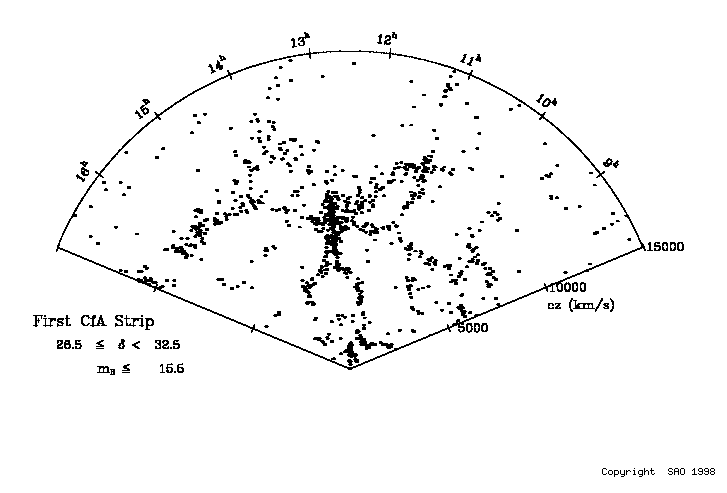
\includegraphics[width=\textwidth]{figures/theory/cfa.png}
\caption{CfA Redshift Survey result showing the distribution of galaxies in a strip on the sky about 6 degrees wide and 130 degrees long. The radial coordinate is redshift, in km/sec, calculated with a Hubble constant of 20km/sec/million ly. Figure from \cite{cfasite}. }
\label{fig:cfa}
\end{center}
\end{figure}


\section{Evidence for Dark Matter}
The previous section gave an overview of why \ac{CDM} as become, over the last century, the leading paradigm to explain the small and large-scale structure observed in our universe. The following subsections deal with particular pieces of evidence, discussed in detail.

\subsection{Galaxies and Clusters}
Galactic rotation curves were discussed above as evidence for dark matter halos. Here we further discuss the properties of dark matter halos. An example of a galactic rotation curve of a spiral galaxy showing the presence of an inferred dark matter halo is shown below in Figure~\ref{fig:rot_curve}. Each side of  Figure~\ref{fig:rot_curve} shows the same galaxy, NGC 3198, but fit with a different disk and halo model. In this particular example from 1985, the authors note their uncertainty about which halo model is the correct one: ``Should one seriously consider the case where the amount of visible matter is negligible with respect to the amount of dark matter [Figure~\ref{fig:rot_curve} (left)]? Or is the maximum disk case [Figure~\ref{fig:rot_curve} (right)] closer to the truth?" \cite{Albada1985}. A decade later, in 1996, Navarro, Frenk and White published a paper describing high-resolution simulations of \ac{CDM}, which could all be fit with a universal dark matter halo profile \cite{Navarro1996}. This formula became known as the \ac{NFW} profile; it is still widely used today, and is the basis for many direct detection experiments, including \ac{LUX}. The \ac{NFW} profile showed that Figure~\ref{fig:rot_curve} (left) is the preferred model, where the amount of dark matter far outweighs the amount of visible matter.

\begin{figure}[htbp]
\begin{center}
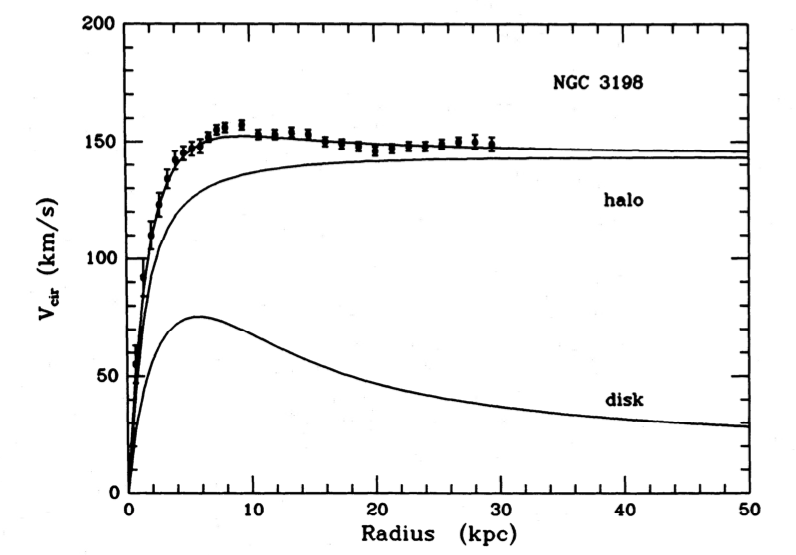
\includegraphics[width=\halffig]{figures/theory/rot_curve2.png}
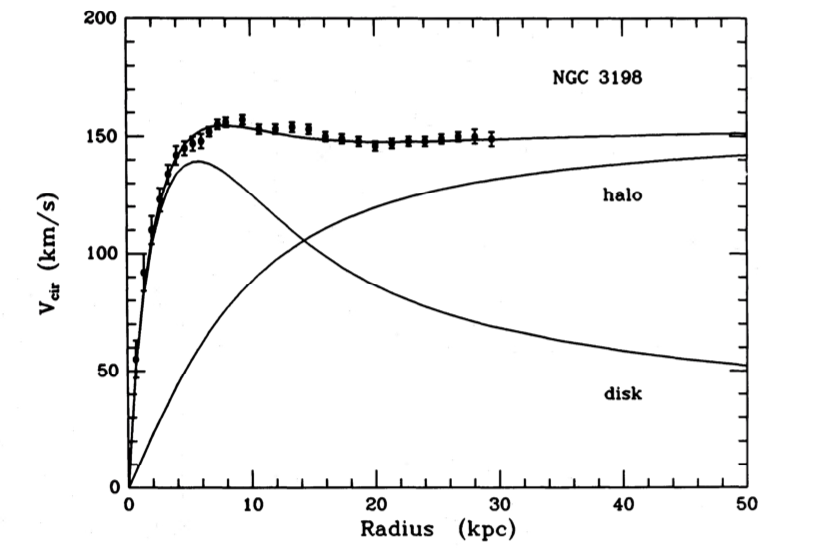
\includegraphics[width=\halffig]{figures/theory/rot_curve1.png}
\caption{Galactic rotation curve from \cite{Albada1985} fit with two different dark matter halo models. The Figure (left) is closer to the rotation curve produced by dark matter with an \acs{NFW} profile (see \cite{Navarro1996}), and our understanding of the ratio of dark matter to visible matter in most spiral galaxies. }
\label{fig:rot_curve}
\end{center}
\end{figure}

The astrophysics community is nearly unanimous in agreement that galaxies have a dark matter component. Today, research continues into the particular shape of the dark matter profile. While \ac{NFW} is in common use and agrees with many observations, it is not consistent with observations of low surface brightness and dwarf galaxies \cite{DeBlok2001}, \cite{DeBlok2001a}. This known as the core-cusp problem: \ac{NFW} galaxies have an over-density of dark matter at small radius (cuspy), while dwarf galaxies favor flatter density profiles (core). Some argue that such behavior may be a consequence of the nature of dark matter, or that current simulations are not sufficient to properly understand dwarf galaxies \cite{Oman2015}. Others argue that a cusp can be changed to a core via baryonic feedback that arises in simulations of active galactic nuclei \cite{Martizzi2013}. 

Other current research into dark matter halos centers on the globular clusters and stars that orbit the Milky Way. These researchers look for evidence of halo substructure and streams of dark matter from the movements of stars orbiting the Milky Way. Data from the Gaia satellite, launched in 2013, calls into question whether dark matter halos are truly in equilibrium, which has consequences for direct detection experiments, as it would change the expected dark matter recoil spectrum \cite{Herzog-Arbeitman2018} \cite{Necib2018}. In particular, \cite{Herzog-Arbeitman2018} measures the velocity distribution of the Milky Way from populations of stars with different metallicities, and finds that the empirical velocity distribution is shifted toward lower velocities and has a slightly different shape when compared with the standard halo model. See Figure~\ref{fig:halo_model_vs_data} for the velocity distributions and the inset for the effect on the resulting zero background limits.

\begin{figure}[htbp]
\begin{center}
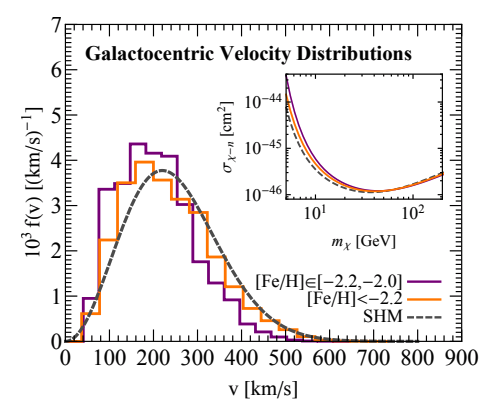
\includegraphics[width=0.8\textwidth]{figures/theory/halo_model_vs_data.png}
\caption{Galactocentric speed distributions for SDSS stars within 4~kpc of the Sun and distances of 7 < r < 10~kpc. The distributions are shown for [Fe/H] in [-2.2, -2] (solid purple) and [Fe/H] < -2.2 (solid orange). The Standard Halo Model with mean $v_{0}$ = 220~km/s is shown for comparison (dashed gray). The inset shows the expected background-free 95\% C.L. limit on the \acs{DM} spin-independent scattering cross section, assuming the exposure and energy threshold of the \acs{LUX} experiment different velocity distributions. Figure from \cite{Herzog-Arbeitman2018}. }
\label{fig:halo_model_vs_data}
\end{center}
\end{figure}

In addition to the stars and globular clusters orbiting the Milky Way, there could be clusters of dark matter more dense than the surrounding halo. Telescope data shows evidence for dark matter halo substructure in the Milky Way \cite{Erkal2017}, and simulations expect upcoming data from LSST to further contribute to the understanding of Milky Way halo substructure and rule out or confirm certain dark matter halo models \cite{Banik2018}.

Galaxy clusters make up some of the strongest direct evidence for dark matter though the method of gravitational lensing. A gravitational lens is created when a massive object is located between a light source and an observer. General relativity requires photons to propagate on the null geodesics of spacetime, meaning the path the light takes from the source will be bent by the distorted space-time of the the massive object. Thus images of background galaxies are distorted by invisible mass along the line of sight from the observer. Being dependent on general relativity, and therefore Newtonian dynamics, the numerous observations of gravitational lensing in large structures strongly disfavor \ac{MOND}. 

There are three types of gravitational lensing: strong, weak, and microlensing. Weak lensing has been used to observe dark matter in large scale structures (galaxy clusters); the other types of lensing are not treated here. In weak lensing, the light sources are far away from the foreground mass (or the mass is small). Several light sources are required, and the location of the mass is statistically reconstructed. The Bullet Cluster (1E0657-558) is one of the most dramatic weak lensing measurements to date: it is actually the collision of the galaxy cluster 1E0657-56 and smaller cluster (the ``bullet") \cite{Markevitch2001}. The x-ray image of the collision, by the Chandra x-ray observatory, shows the location of the baryonic matter. The baryonic matter suddenly slowed down upon the collision, emitting shock x-rays  \cite{Markevitch2001}. The authors of \cite{Markevitch2001} call it ``a textbook example of a bow shock", indicating the x-ray behavior is well understood. A few years later, Clowe et al. also call the Bullet Cluster ``a direct empirical proof of the existence of dark matter" \cite{Clowe2006}. Their weak lensing observations show the location of the total mass centers of the two clusters to be offset from the location of the baryonic matter at a significance of 8$\sigma$ \cite{Clowe2006}. In the collision, the dark matter halos of the two clusters pass through each other without slowing down, while the baryonic matter in the two clusters interacts, slowing down dramatically and producing x-rays. The weak lensing measurement is shown overlaid with the visible and x-ray images in Figure~\ref{fig:bullet}. Such a dramatic offset cannot be explained by modifications to gravity. It is important to note that there are many lensing measurements that show a statistically significant offset between baryonic matter and total matter; the Bullet Cluster is just one example, albeit particularly dramatic.

\begin{figure}[htbp]
\begin{center}
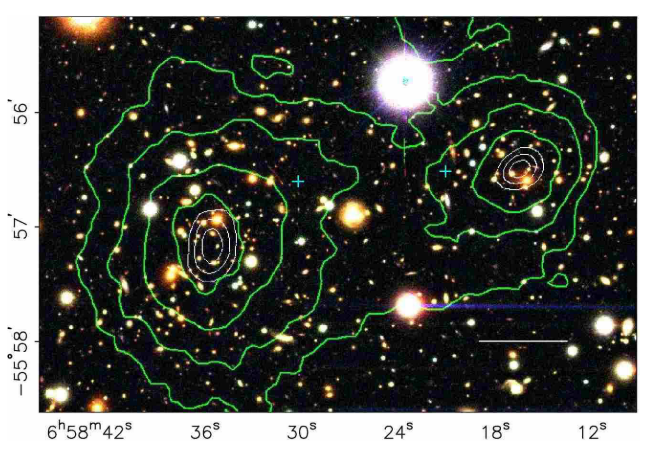
\includegraphics[width=\halffig]{figures/theory/bullet1.png}
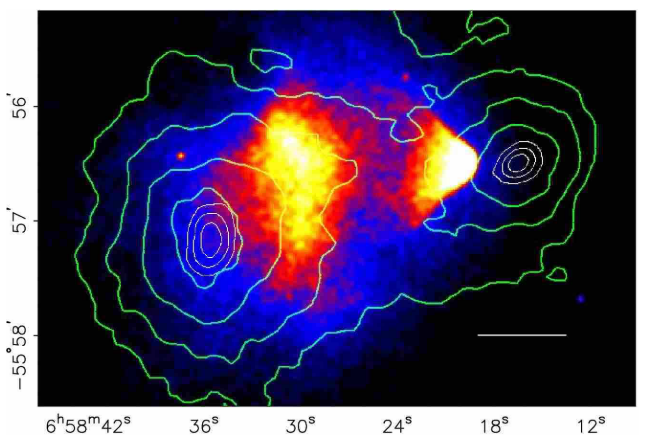
\includegraphics[width=\halffig]{figures/theory/bullet2.png}
\caption{(left) The visible light image from the Magellan telescope of the merging Bullet Cluster overlaid with the weak lensing measurement contours in green, and white 68.3\%, 95.5\%, and 99.7\% confidence levels for the weak lensing peaks. (right) The Chandra x-ray image overlaid with the same weak lensing measurement. Figure from \cite{Clowe2006}. }
\label{fig:bullet}
\end{center}
\end{figure}


\subsection{Cosmic Microwave Background}
\label{sec:cmb_dm}
In the thermal history of our universe, the term recombination refers to the epoch when temperatures had cooled enough to allow electrons and protons to combine into hydrogen, leaving photons to propagate freely through the universe. The photons should have decoupled from the matter as a black body peaked at the temperature of recombination,  $\approx$3000~K. The relic radiation from this epoch is visible today as the \ac{CMB}, where the continuing expansion of the universe has redshifted the peak of the black body spectrum to $\approx$2.7~K. The \ac{CMB} photons are also referred to as the light of last scattering, referring to the interaction the photons had with free electrons before the electrons became bound to protons in hydrogen. The temperature of the \ac{CMB} was precisely measured to be 2.7377 $\pm$ 0.0038~K  by the COBE mission, which also confirmed its perfect adherence to a black body spectrum \cite{Smoot1999} (Figure~\ref{fig:cobe}).

\begin{figure}[htbp]
\begin{center}
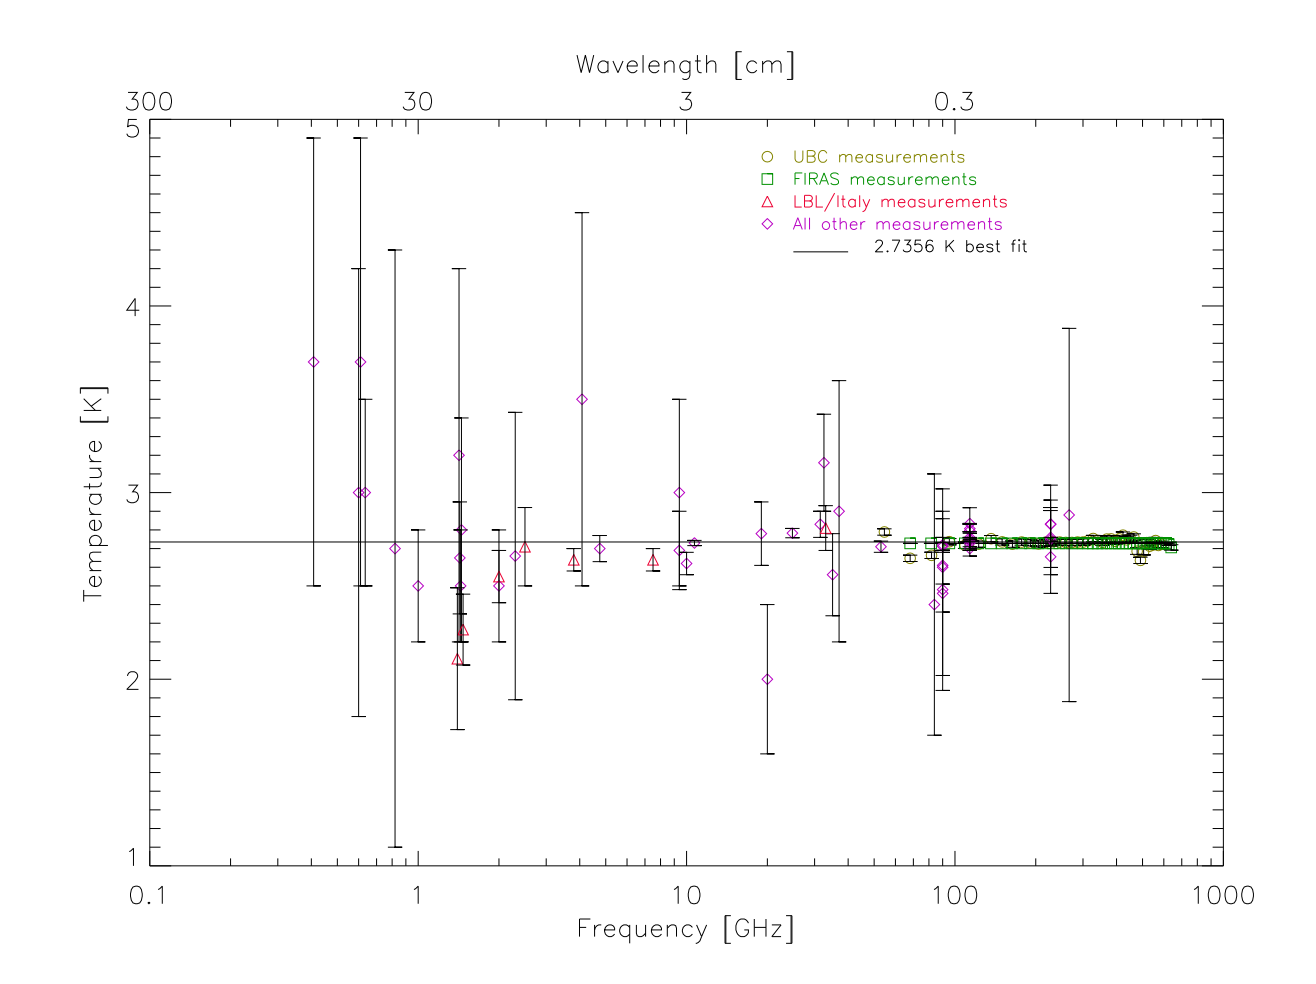
\includegraphics[width=\textwidth]{figures/theory/cobe_temp.png} \\
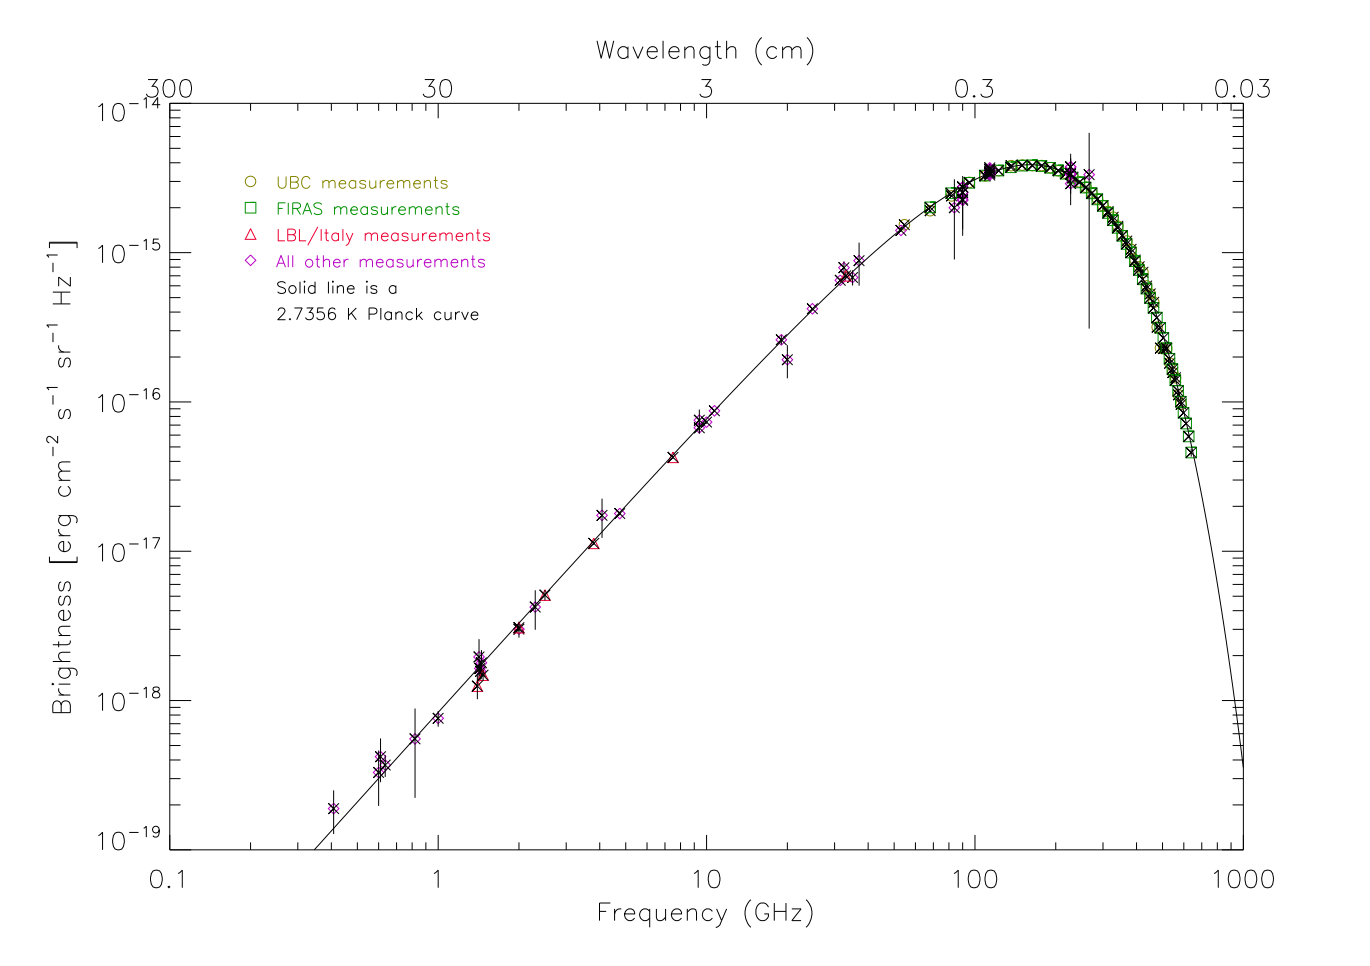
\includegraphics[width=\textwidth]{figures/theory/cobe_spectrum.png}
\caption{(top) The FIRAS instrument on the COBE satellite mission measured the \acs{CMB} temperature to be 2.7377 $\pm$ 0.0038~K. (bottom) The FIRAS instrument also confirmed the perfect Planck black body spectral shape of the \acs{CMB} radiation. Figures from \cite{Smoot1999}. }
\label{fig:cobe}
\end{center}
\end{figure}

While the COBE satellite mission's measurements of the \ac{CMB} provided strong support for the Big Bang model of cosmology, it was COBE's discovery of anisotropies in the \ac{CMB} that eventually led to powerful evidence for \ac{CDM}. Since COBE, two more \ac{CMB} satellite missions, WMAP and Planck, have launched and gathered data, each with successively higher spatial and energy resolution. The relative resolutions of COBE, WMAP, and Planck are shown in Figure~\ref{fig:cmb} along with the full Planck \ac{CMB} anisotropy map. The scale of the anisotropy fluctuations represent a scale of  $\pm$~30~$\mu$K; the \ac{CMB} power spectrum remains the most perfect black body spectrum observed in nature. 

\begin{figure}[htbp]
\begin{center}
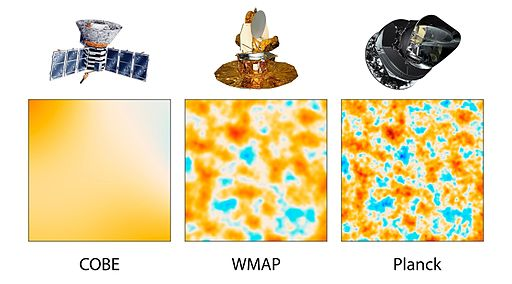
\includegraphics[width=.6\textwidth]{figures/theory/satellites.jpg}
\includegraphics[width=\textwidth]{figures/theory/planck.png}
\caption{(top) The relative spatial resolution of COBE, WMAP, and Planck. Figure courtesy of NASA. (bottom) The Mollweide projection of the Planck 2013 CMB temperature map. The color scale represents fluctuations of $\pm$~30~$\mu$K around a central value of 2.7377~K. Figure courtesy of ESA and the Planck Collaboration. }
\label{fig:cmb}
\end{center}
\end{figure}

The fluctuations $\Delta T(\theta, \phi)$ of the \ac{CMB} map shown in Figure~\ref{fig:cmb} can be decomposed into its basis components via Fourier analysis, where each expansion component is represented by the spherical harmonics, $Y_{lm}$:

\begin{equation}
\label{eq:cmb_fluct}
\Delta T(\theta, \phi) = \sum_{l=2}^{\infty} \sum_{m=-l}^{l} b_{lm} Y_{lm}(\theta, \phi)
\end{equation}
The sum leaves out the $l=0$ (mean) and $l=1$ (dipole Doppler shift caused by movement of the earth with respect to the \ac{CMB}) components, which were subtracted from the \ac{CMB} temperature map, leaving only the fluctuations as in Figure~\ref{fig:cmb}. The power spectrum of the temperature fluctuations, which is calculated by squaring Equation~\ref{eq:cmb_fluct}, averaging it over all points that have the same angular separation $\theta$, and performing an integral over all $m$ (because the temperature anisotropies have no preferred direction), encodes all the statistical variation in the \ac{CMB} sky (see, e.g. \cite{Hu2008} for a derivation). The angular correlations of the different multipole moment $l$ are typically extracted from this power spectrum and plotted as function of $l$ and the coefficients $C_{l}$ from the power spectrum. This quantity is referred to as the angular power spectrum and takes the form:

\begin{equation}
D_{l}^{TT} = \frac{ l(l + 1)}{ 2 \pi} C_{l}
\end{equation}
where the $TT$ superscript denotes temperature anisotropies (polarization anisotropies, not discussed here, can be parameterized similarly). The latest angular power spectrum from Planck is shown in Figure~\ref{fig:planck_multipole}.

\begin{figure}[htbp]
\begin{center}
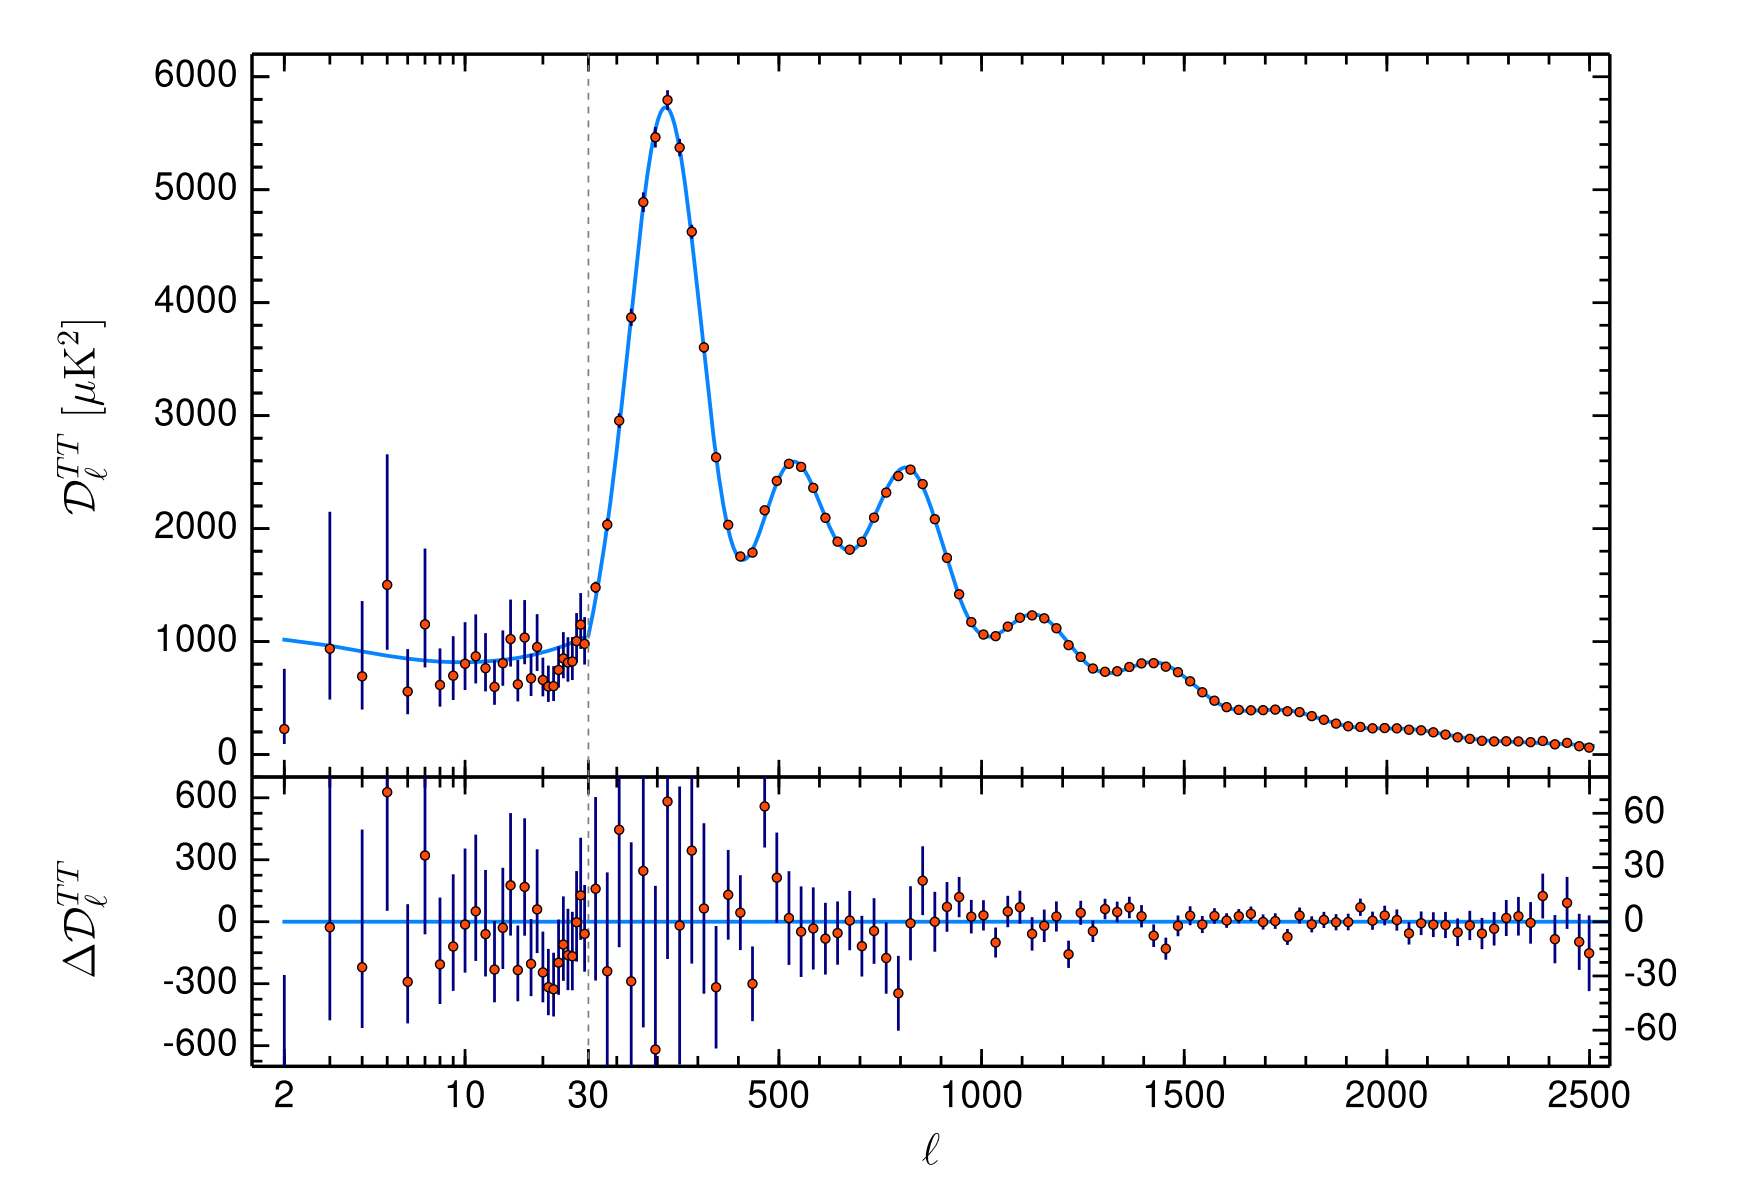
\includegraphics[width=\textwidth]{figures/theory/planck_multipole.png}
\caption{The angular power spectrum from Plank 2018 results  \cite{Planck2018}. }
\label{fig:planck_multipole}
\end{center}
\end{figure}

The location and magnitude of peaks in the angular power spectrum (Figure~\ref{fig:planck_multipole}), constrain the curvature, content, and evolution of our universe. The physical interpretation of the \ac{CMB} fluctuations is as follows: photons from the time of last scattering, newly free to propagate through the universe, carry information about the density fluctuations in the plasma from which they decoupled. The plasma, which was then composed of photons, baryons, and dark matter, behaved as an oscillator driven by gravitational attraction, with a restoring force from the fluid pressure of the plasma. The maxima of the angular power spectrum indicate extrema, overdensities or underdensities, in the plasma. The presence of baryons increases the magnitude of odd peaks relative to even peaks. The physical interpretation of this is that baryons add inertia to the oscillator system, causing an increase in compression (odd) compared to expansion (even) \cite{Hu2008}. The angular power spectrum peaks are sometimes referred to acoustic peaks, as the oscillations that produced them were longitudinal and depended on density, much like sound waves. The presence of dark matter is apparent in the relative heights of the second and third peak in the spectrum. The driving force of the oscillator is the total matter content (baryons + dark matter,) which contributes to odd peaks, while baryons contribute characteristically to the even peaks. A third peak that is similar or larger than a second peak indicates that the matter content at the time of recombination was dominated by dark matter. A useful demonstration of the effect of baryons and total matter on the angular power spectrum is shown in Figure~\ref{fig:matter_baryons}.

\begin{figure}[htbp]
\begin{center}
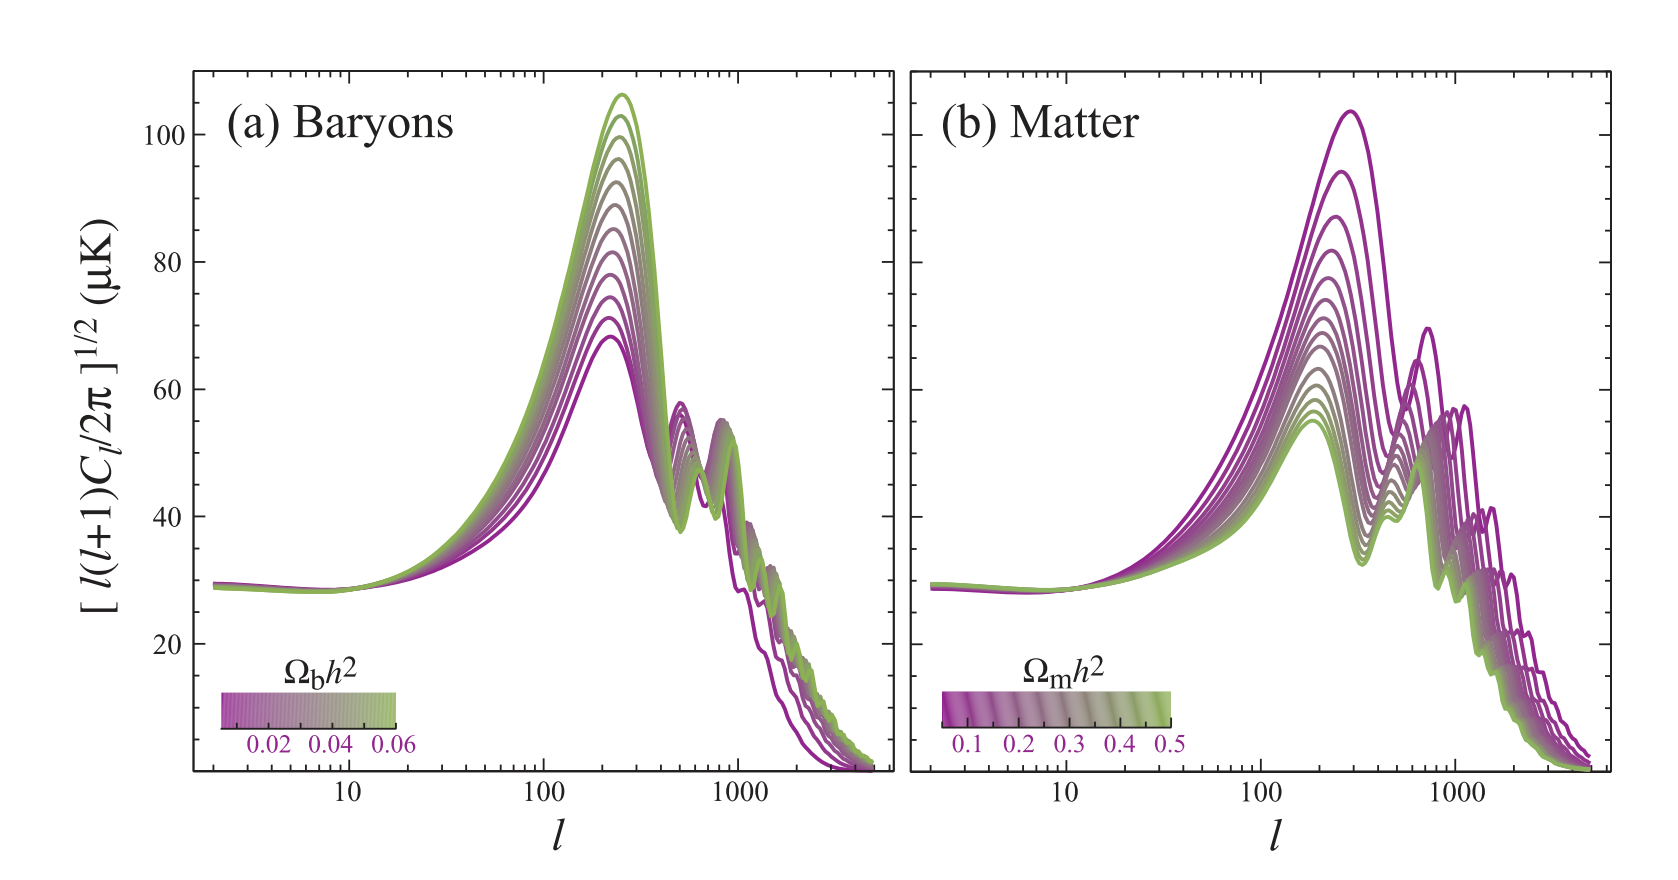
\includegraphics[width=\textwidth]{figures/theory/matter_baryons.png}
\caption{The effect of baryons (left) and total matter (right) on the magnitude and location of \acs{CMB} angular power spectrum peaks.  \cite{Hu2008} }
\label{fig:matter_baryons}
\end{center}
\end{figure}

The measure of the dark matter content and baryon content of today's universe can be extrapolated from fitting the \ac{CMB} angular power spectrum as in Figure~\ref{fig:matter_baryons}. The results from the Planck 2018 angular power spectrum (\cite{Planck2018}) are: 

\begin{equation}
\Omega_{cdm} = 0.2696 \pm 0.0047
\end{equation}

\begin{equation}
\Omega_{b}  = 0.0495 \pm 0.0005 
\end{equation}
where the subscript $b$ refers to baryon and the subscript $cdm$ refers to cold dark matter. Each $\Omega_{x}$, defined in more detail below, represents the fraction of today's mass-energy density comprised by constituent $x$. These values do not add to one because a large fraction of the mass-energy density of the universe is comprised of dark energy, which we have left discussion of until the next section. However, note that these two values alone measure dark matter to comprise \~84\% of the matter in our universe. 


%; $h$ is the dimensionless version of the Hubble constant, $H_{0}$, which is the dominant source of error in these measurements. The Hubble constant $H_{0}$ is the ratio of the expansion of the universe to its size at $t=t_{0}$ (today). 

\section{Standard Models}
Thus far we have focused only on the astrophysical and cosmological evidence for particle \ac{CDM}. \ac{CDM} plays a central role in the standard model of cosmology, known as \ac{LCDM}. In this section, we briefly summarize the standard models of cosmology and particle physics. 


% $\Lambda$\ac{CDM} (``Lambda'' - \ac{CDM}). 
\subsection{The Standard Cosmology}
The standard \ac{LCDM} cosmology is based on the Einstein field equations:

\begin{equation}
R_{\mu \nu} - \frac{1}{2} g_{\mu \nu} R = \frac{8 \pi G}{c^{4}} T_{\mu \nu} + \Lambda g_{\mu\nu}
\end{equation}
where $R_{\mu \nu}$ is the Ricci tensor, $R$ is the Ricci scalar, and $g_{\mu\nu}$ is the metric tensor. $T_{\mu \nu}$ is the stress-energy tensor, $G$ is Newton's gravitational constant, $c$ is the speed of light in vacuum, and $\Lambda$ is the cosmological constant. The equation relates the geometry of space-time (on the left hand side) to the energy content of the universe (on the right hand side). 

Einstein originally introduced the cosmological constant $\Lambda$ to counteract gravity and produce a steady-state universe. Today, however, we know that the universe is expanding, and that the rate of expansion is accelerating. The second fact, first evidenced by supernova Type Ia measurements \cite{Riess1998} \cite{Perlmutter1998}, is what led to the modern interpretation of $\Lambda$ as dark energy. Today, we understand  $\Lambda$ to represent a ``vacuum energy'' associated with space-time itself, rather than its matter content. It is the source of the accelerating expansion of the universe, sometimes referred to as ``negative pressure'' or ``gravitational repulsion'', and it is the dominant component of mass-energy density in our universe (see Table~\ref{tb:planck}).

The Einstein field equations are solved with the Friedman-Lemaitre-Robertson-Walker metric (not shown here, see e.g. \cite{Ryden2006}, \cite{Kolb1990}), which describes the symmetries we observe in our universe and therefore require of our model: isotropy and homogeneity. The solution yields the Friedman equation (Equation~\ref{eq:friedman}), which details how the addition of different energy sources (matter, radiation, dark energy) change the expansion rate of the universe. The rate of expansion is given by the Hubble constant $H(t)$ (a slight misnomer because it can change over time scales $\sim$ history of our universe). It is defined as $H(t)^{2} \equiv \frac{\dot{a}(t)}{a(t)}$, where $a$ is the so-called scale factor, which is a dimensionless factor that parametrizes the size of the universe. The Friedman equation, given below, delineates how the Hubble constant changes with the energy content $\rho_{tot}$ and curvature $k$ of our universe.

\begin{equation}
\label{eq:friedman}
H(t)^{2} \equiv \Big( \frac{\dot{a}(t)}{a(t)} \Big) = \frac{8 \pi G}{3} \rho_{tot}(t) - \frac{k}{a(t)^{2}}
\end{equation}
The Friedman equation yields a quantity known as the critical density $\rho_{c}$, which is the density for a flat universe ($k=0$). 

\begin{equation}
\rho_{c}(t) = \frac{ 3 H(t)^{2}}{8 \pi G} 
\end{equation}
A species $x$ is defined as having a fraction of the mass-energy density $\Omega_{x}(t) = \rho_{i}(t) / \rho_{c}(t)$. The individual $\Omega_{x}$ have different time evolutions according to their equation of state (see e.g. \cite{Ryden2006}, \cite{Kolb1990}, for a complete, pedagogical treatment). After treating equations of state, the Friedman equation can be re-written in a more convenient form: 

\begin{equation}
\label{eq:Lcdm}
\frac{H^{2}}{H_{0}^{2}} = \frac{\Omega_{r, 0}}{a^{4}} + \frac{\Omega_{m, 0}}{a^{3}} + \Omega_{\Lambda, 0} + \frac{( 1 - \Omega_{tot,0})}{a^{2}} 
\end{equation}
where the $0$ subscript denotes today's value, $r$ denotes radiation, $m$ denotes matter, and $\Lambda$ denotes dark energy. Note that the last term disappears when $\rho_{0} = \rho_{c}$, that is, if our universe is flat. Equation~\ref{eq:Lcdm} makes a powerful statement: by measuring the energy content of the universe, we can tell the history and fate of the Universe. This is the core of\ac{LCDM} -- it is essentially a system of equations, which, when solved, can describe the history and predict the future of the universe in terms of a few measurable parameters (e.g $\Omega_{x}$). 

The Planck collaboration fits for a standard, 6 parameter \ac{LCDM} of the \ac{CMB}. This fit includes some parameters specific to the intricacies \ac{CMB} measurements, as well as the familiar $\Omega_{x}$ density parameters from Equation~\ref{eq:Lcdm}. The 6 fit parameters\footnote{ The density parameters are often reported as $\Omega_{x}h^{2}$ since the main source of error in their measurement comes from the Hubble constant $H_{0}$. $h$ is a dimensionless parameter defined as: $h = H_{0}/( 100~km~s^{-1}~Mpc^{-1})$} are:  $\Omega_{b}h^{2}$, $\Omega_{cdm}h^{2}$, $\tau$, ln$(10^{10}A_{s})$, $n_{s}$, and $100\theta_{MC}$. Other quantities are derived from these parameters. A summary of the parameters, derived quantities, and their values is given in Table~\ref{tb:planck}. Note that the parameter $A_{s}$ is the amplitude of curvature fluctuations in the \ac{CMB} angular power spectrum (Figure~\ref{fig:planck_multipole}). The effect of baryons and dark matter on the angular power spectrum were discussed in Section~\ref{sec:cmb_dm}. Similarly, dark energy content, curvature, and equation of state of the universe also produce visible effects (see examples in Figure~\ref{fig:curve_etc}). Namely, dark energy and curvature determine the magnitude of the first peak, and curvature determines peak locations.

\begin{figure}[htb]
\begin{center}
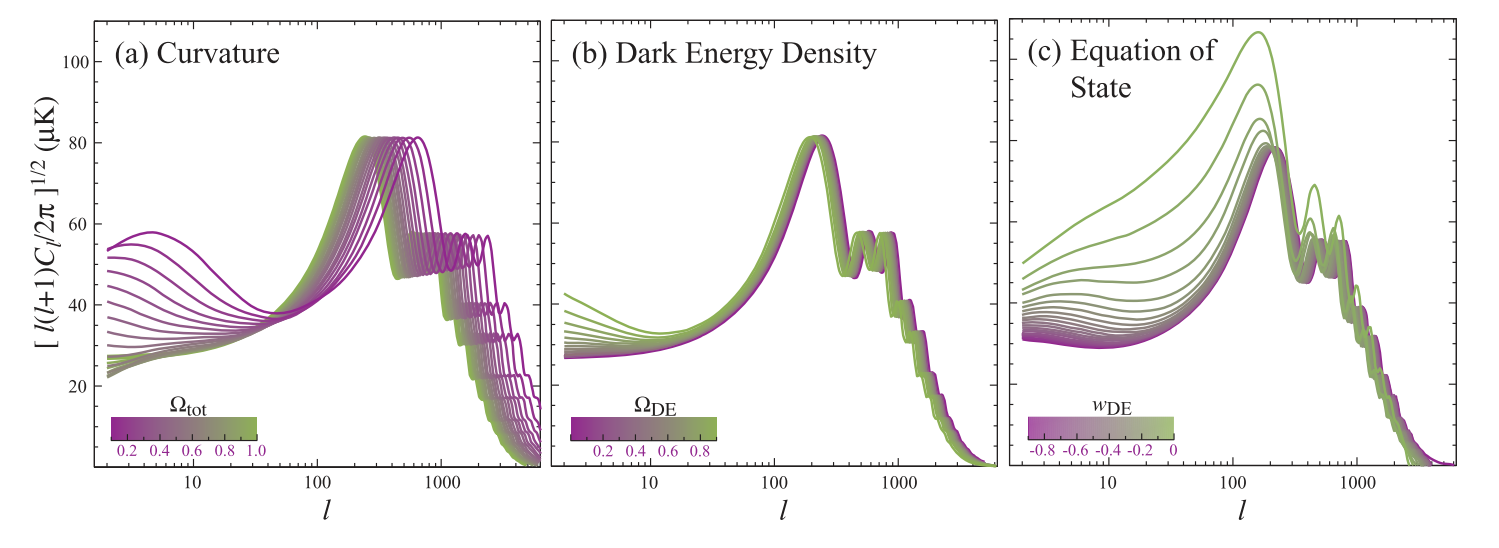
\includegraphics[width=\textwidth]{figures/theory/curve_etc.png}
\caption{The effect of curvature (left), dark energy (center), and equation of state (right) on the magnitude and location of \acs{CMB} angular power spectrum peaks.  \cite{Hu2008} }
\label{fig:curve_etc}
\end{center}
\end{figure}


\begin{table}[htbp]
\caption{A summary of the fit parameters and derived quantities from Planck's 2018 results \cite{Planck2018}.}
\begin{center}
\begin{tabular}{ r l c }
\hline
Fit Parameter & Definition &  Planck TT spectrum \\
\hline
$\Omega_{b}h^{2}$ & baryon density & 0.02212 $\pm$ 0.00022 \\
$\Omega_{cdm}h^{2}$ & CDM density & 0.1206 $\pm$ 0.0021 \\
$100\theta_{MC}$ & angular acoustic scale & 1.04077 $\pm$ 0.00047 \\
$\tau$ & optical depth & 0.0522 $\pm$ 0.0080 \\
ln$(10^{10}A_{s})$ & curvature fluctuations & 3.040 $\pm$ 0.016 \\
$n_{s}$ & spectral index & 0.9626 $\pm$ 0.0057 \\
\hline
Derived Quantity & Definition &  Planck TT spectrum \\
\hline
$\Omega_{b}$ & baryon content & 0.0495 $\pm$ 0.0005 \\
$\Omega_{cdm}$ & CDM content & 0.2696 $\pm$ 0.0047 \\
$\Omega_{m}$  & matter content & 0.321 $\pm$ 0.013 \\
$\Omega_{\Lambda}$  & dark energy content & 0.679 $\pm$ 0.013 \\
$H_{0}$ [km~s$^{-1}$~Mpc$^{-1}$] & Hubble constant & 66.88 $\pm$ 0.92 \\
Age [Gyr]  & age of the universe & 13.830 $\pm$  0.037 \\
$k$ & curvature & consistent w/ $k=0$ \\
\label{tb:planck}
\end{tabular}
\end{center}
\label{default}
\end{table}%


\FloatBarrier
\subsection{The Standard Model of Particle Physics}
The \ac{SM} of particle physics describes all the currently known matter particles and force carrier particles, which can also have mass, and which dictate interactions between the matter particles. As of 2012, it also includes a mass generation mechanism from the Higgs boson. The \ac{SM} is formulated using the principles of Quantum Field Theory, where symmetries in the Lagrangian give rise to conserved physical quantities and thereby determine the rules for interactions.

\begin{figure}[htbp]
\begin{center}
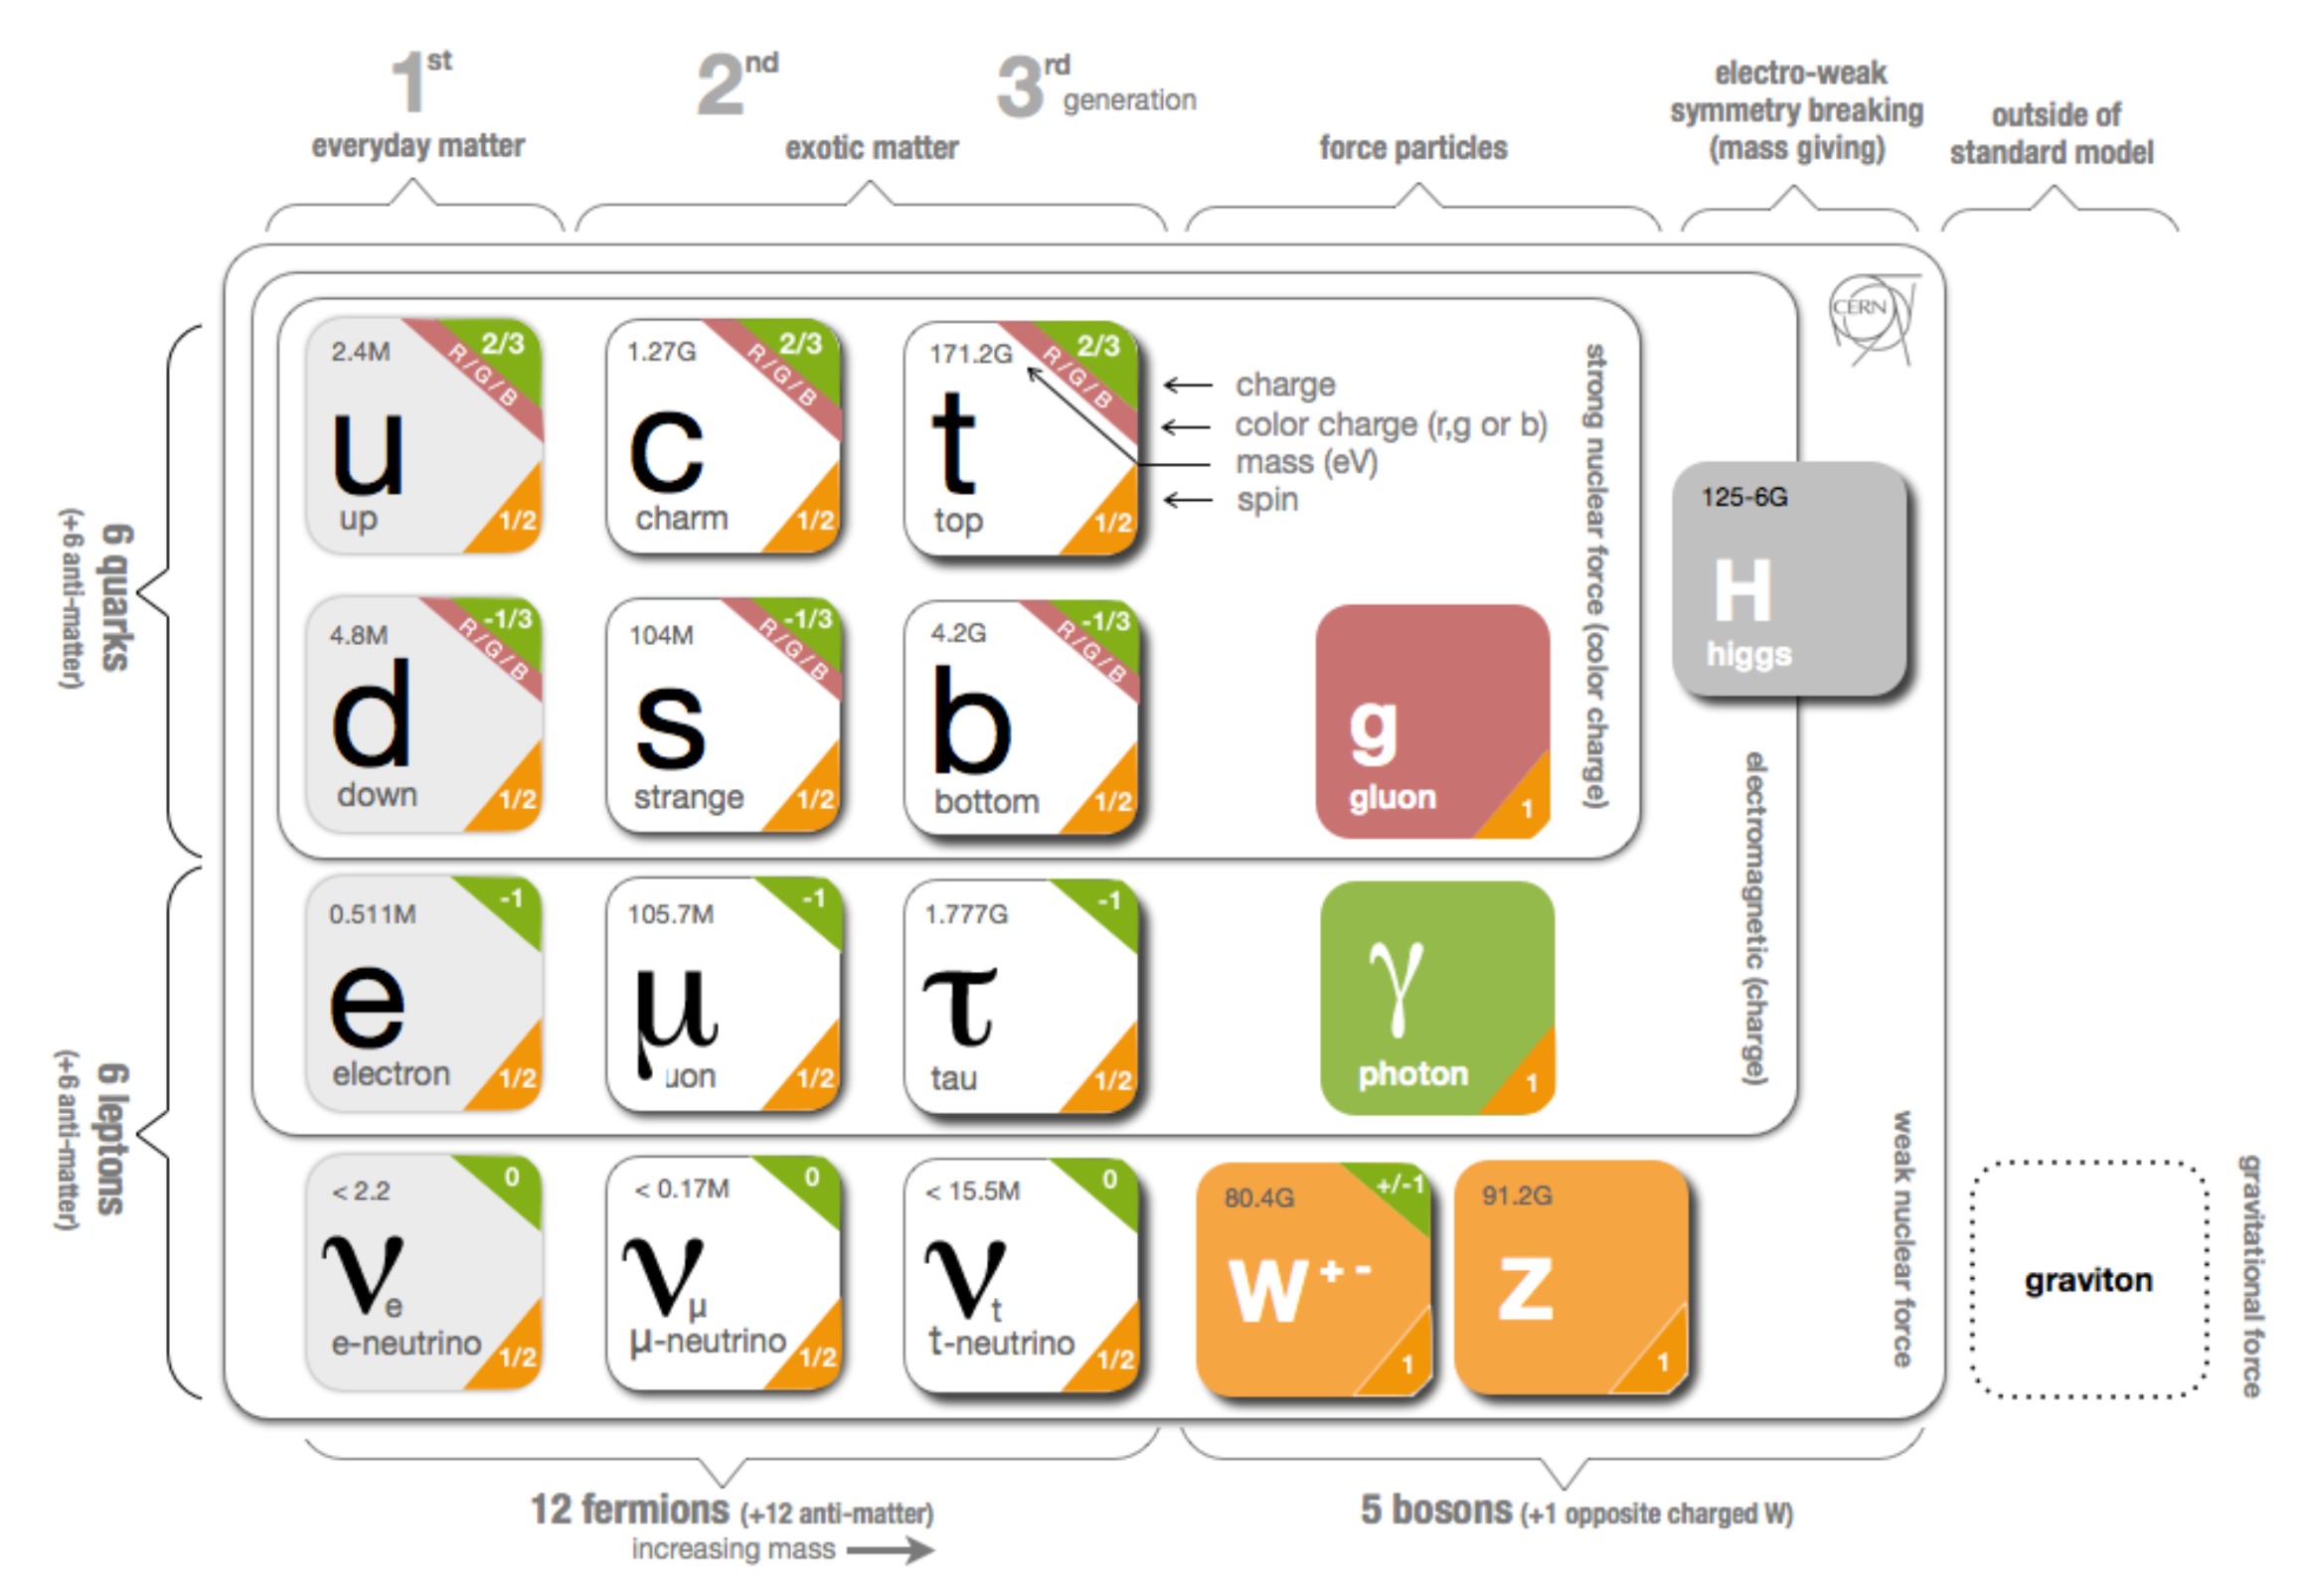
\includegraphics[width=\textwidth]{figures/theory/sm.png}
\caption{The particles that comprise the standard model of particle physics, including names, spins, masses, and charges. It is also indicated which fermions interact with which bosons, e.g. gluons interact with the quarks but not with the leptons. }
\label{fig:sm}
\end{center}
\end{figure}


The known particles of the \ac{SM} are shown in Figure~\ref{fig:sm}, along with a theoretical force carrier for gravity, the graviton. These particles are typically grouped into categories: fermions and bosons. Fermions comprise all the known matter particles and are spin-$\frac{1}{2}$ particles. Each of the fermions in Figure~\ref{fig:sm} has an anti-particle, although it is an open question whether the neutrino is its own anti-particle. The integer-spin bosons, excepting the Higgs boson, which provides a mechanism for giving mass to all the other particles, are the force carriers of the standard model. The spin-1 bosons: the gluon, photon, and $W$ and $Z$ boson, describe three of the four forces known to physics. The gluon mediates the strong force, which governs interactions between quarks, binding them in hadrons (three quark states which make up e.g. protons and neutrons) and mesons (two-quark states such as pions). The photon mediates electromagnetism, governing interactions between particles with electric charge. The $W^{+}$, $W^{-}$, and $Z$ bosons mediate the weak force, which includes phenomena such as beta-decay and neutrino-electron scattering.

It was once proposed that the $Z$ boson could mediate the interaction between \ac{DM} and \ac{SM}, because a \ac{DM} particle that interacts via the weak force fits the \ac{WIMP} paradigm discussed below. Direct detection experiments have long excluded the scattering cross section, of $\~10^{-39}$~cm$^{2}$, which is the cross section for an O(1) coupling to the Z. It should be noted that some extensions to the \ac{SM} allow for $<$ O(1) coupling to the Z via, e.g., a mixing angle \cite{Cheung2013}. Naively, it is possible for neutrinos, which interact weakly and have mass, to be \ac{CDM}. However, neutrinos were relativistic during structure formation so could not perform the role of necessary of \ac{CDM}. Estimates of the density of today's relic neutrinos show that $\Omega_{v} \approx (1.2 - 2.2) \times 10^{-3} << \Omega_{cdm}$ \cite{Quigg2008}, \cite{Hannestad2004}. The standard model, as it is known today, contains no particles that could be \ac{CDM}. 

\section{Dark Matter Candidates Motivated by Particle Physics}
Cosmology, while providing very precise measurements of the dark matter content of the universe, essentially requires only three things of dark matter candidates: (1) the candidate must account for the observed $\Omega_{cdm}$, (2) at least 95\% of it is non-relativistic or ``cold'' \cite{Viel2005}, (3) it is not strongly self-interacting (``collisionless'') or strongly interacting with baryons. Requirement (1) is fairly loose, as it is possible for multiple different dark matter particles to comprise together $\Omega_{cdm}$, but note that it implies the dark matter candidate(s) must be stable on the timescale of the universe, or there must be a production mechanism to create the necessary abundance seen today. This section briefly summarizes two very different dark matter candidates, which have additional motivation due to open questions from the standard model. 

\subsection{WIMPs and the Hierarchy Problem}
\label{sec:wimp_miracle}
Any system that describes particle interactions today at ``low energy'', should also scale to describe particle interactions at different times (and therefore energies) in the history of our universe, namely in the first 10$^{-43}$ seconds after the Big Bang in a time known as the Planck epoch. During the Planck epoch, energies were at the Planck scale of $10^{19}$~GeV, and gravitational interactions become as large as the other forces. Any sound quantum theory should be able to account for interactions at this energy scale. However, the largest masses for \ac{SM} particles are O(100)~GeV; this scale is known as the weak scale and is 17 orders of magnitude less than the Planck scale. The hierarchy problem is essentially a question of why the Higgs mass is so much lighter than the Planck mass. If one tries to calculate the Higgs mass the usual way, by summing all the loop contributions to the two point function, the sum diverges. This is in contrast to the measured mass, which is about 125~GeV. 

%is the known as the electroweak scale, when electromagnetism and the weak force unify. The breaking of the electroweak symmetry is done by the Higgs mechanism, which provides mass. There is a compelling argument that the strong and electroweak forces unify at energies referred to as the \ac{GUT} scale, and that this theory then unifies with gravity at the Planck scale (sometimes called ``Theory of Everything'') \cite{Dimopoulos1991}. The 16 orders of magnitude between the Planck scale and the electroweak scale is known as the Hierarchy Problem; there must be new physics between the electroweak scale and the Planck scale, i.e new particles with $m > m_{Higgs}$ and new symmetries, to properly describe particle interactions during the history of our universe.

In order to solve the Hierarchy Problem, a framework known as \ac{SUSY} was developed. In \ac{SUSY} each \ac{SM} particle has a ``superpartner.'' In general, the superpartners have a spectrum of masses higher than \ac{SM} particles and a symmetry called $R$-parity partitions and limits interactions between \ac{SM} and \ac{SUSY}. The superpartners add additional diagrams to the radiative corrections for the Higgs mass. These new contributions stabilize the calculation, cancelling the divergence and resulting in a finite value for the Higgs mass. The connection between \ac{SUSY} and \ac{DM} is that some of these new particles could be dark matter candidates. The lightest of the \ac{SUSY} particles, called the \ac{LSP}, can be stable. If the \ac{LSP} is neutrally charged, then it is a \ac{WIMP} dark matter candidate.

The \ac{WIMP} paradigm has its roots in the mathematical coincidence called the ``\ac{WIMP} Miracle''. If one assumes a weak-scale coupling and mass for dark matter, it naturally produces the entire $\Omega_{cdm}$ observed today via thermal freezeout. When the universe was small and dense with particles, a \ac{WIMP}, $\chi$, would meet its antiparticle $\bar{\chi}$ and annihilate into lighter particles: $\chi \bar{\chi} \rightarrow l \bar{l}$. The reverse reaction to produce the heavier \ac{WIMP} ($ l \bar{l} \rightarrow \chi \bar{\chi} $) proceeds as long as the energies of the particle is sufficiently high, i.e. $T > m_{\chi}$. When this condition is met, the number density $n$ of \ac{WIMP}s is at its thermal equilibrium value $n_{eq}$. As the universe expands, the reaction falls out of thermal equilibrium. Both directions of the reaction ($\chi \bar{\chi} \rightleftharpoons l \bar{l}$) are affected: the reverse reaction cannot produce more $\chi$ due to cooling, and the forward reaction stalls because annihilation rate $\Gamma_{A}$ relies on a sufficiently high number density $n$, such that the probability of $\chi$ to meet $\bar{\chi}$ is large. The number density of \ac{WIMP}s become frozen into a relic density that we can observe today when the Hubble expansion rate overcame the annihilation rate:

\begin{equation}
\begin{split}
H(t) &> \Gamma_{A} \\
 &> n_{\chi} \langle \sigma_{A} v \rangle
\end{split}
\end{equation}
where $\langle \sigma_{A} v \rangle$ is the thermally averaged annihilation cross section. The time when $H(t) = \Gamma_{A}$ is referred to as freezeout. Following \cite{Feng2010}, the time evolution of the number density is described by the Boltzmann equation (see Figure~\ref{fig:wimp_miracle} (left) for number density evolution before and after freezeout):

\begin{equation}
\frac{dn}{dt} = -3 H n - \langle \sigma_{A}v \rangle (n^{2} - n_{eq}^{2} )
\end{equation}
This equation must be solved numerically (a more complete analysis can be found in e.g. \cite{Lisanti2016}), but making a few assumptions, \cite{Feng2010} finds:

\begin{equation}
\begin{split}
\Omega_{\chi} &\sim \frac{m_{\chi} T_{0}^{3}}{ \rho_{c}} \frac{n_{f}}{T_{f}} \\ %\approx  \frac{20 T_{0}^{3}}{ \rho_{c} M_{Pl} } \langle \sigma_{A}v \rangle^{-1}  \end{equation}
&\propto [\mathrm{constants}] \langle \sigma_{A}v \rangle^{-1} 
\end{split}
\end{equation}
where $\rho_{c}$ is the critical density, $f$ subscripts refer to freezeout and $0$ subscripts refer to today's values. $\Omega_{\chi}$ then depends only on the particular annihilation cross section, which is set by the mass scale $m_{\chi}$:

\begin{equation}
\label{eq:sigmav}
\sigma_{A}v = k \frac{g_{weak}^{4}}{16 \pi^{2}m_{\chi}^{2}} ( \mathrm{1~or}~v^{2} ) 
\end{equation}
where $v^{2}$ is present or absent for S- or P-wave annihilation and $k \sim \frac{1}{2} - 2$ parameterizes the deviation of $g$ from $g_{weak} \approx 0.065$. If the mass of the dark matter particle is in the range $m_{\chi} \sim$ 100~GeV-1~TeV, then $\Omega_{\chi}$ accounts for 100\% of today's observed $\Omega_{cdm}$. This is the \ac{WIMP} miracle: weak-scale particles can account for \textit{all} the dark matter content. Even if the \ac{WIMP} mass $m_{\chi}$ deviates from this perfect situation, the particle can still make up a substantial percentage of dark matter (see Figure~\ref{fig:wimp_miracle} (right)),

\begin{figure}[htbp]
\begin{center}
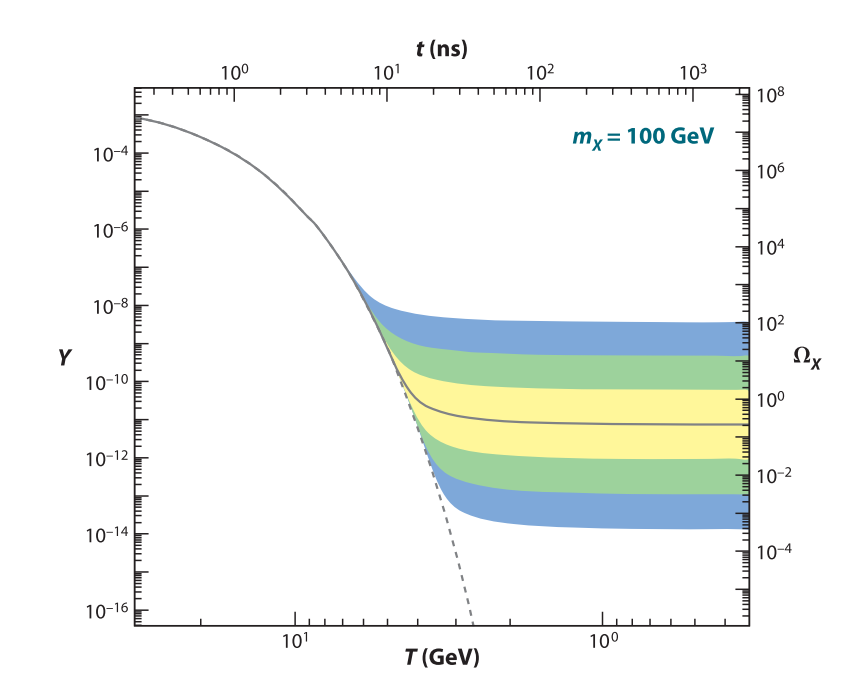
\includegraphics[width=\halffig]{figures/theory/freezeout.png}
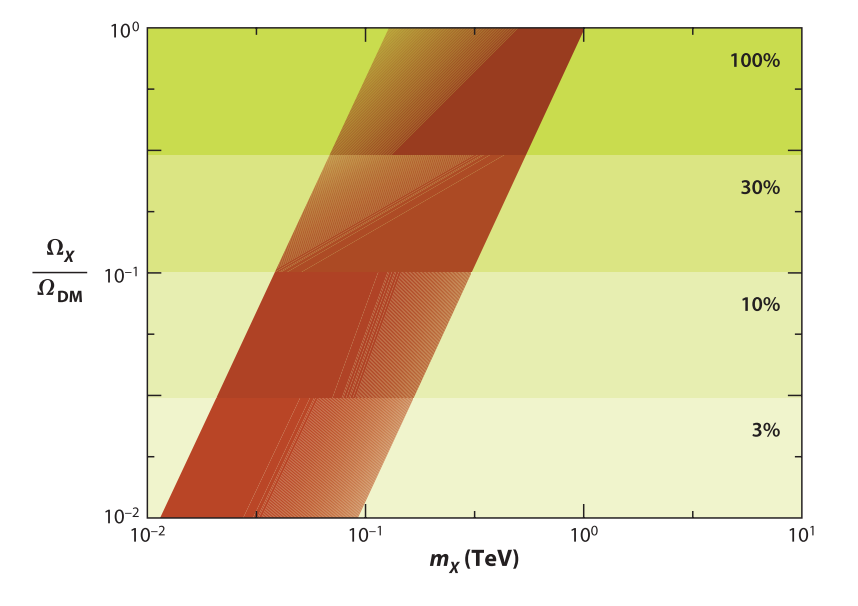
\includegraphics[width=\halffig]{figures/theory/wimp_miracle.png}
\caption{(left) The co-moving number density $Y$ (left y-axis) resulting in the thermal relic density $\Omega_{\chi}$ (right y-axis) for a dark matter particle of mass $m_{\chi}$=100~GeV. The solid black line is the annihilation cross section which yields the correct relic density and bands indicate cross sections that differ by successive factors of 10 from the ``correct'' annihilation cross section. (right) A band of natural values for a thermal relic $\chi$ that composes different percentages of the observed dark matter content. The width of the band is set by the deviation of $g$ from $g_{weak}$ in Equation~\ref{eq:sigmav}. Figures from \cite{Feng2010}}
\label{fig:wimp_miracle}
\end{center}
\end{figure}

A particle with the exact mass and weak-scale coupling, i.e scattering mediation via O(1) coupling with the Z-boson, has been ruled out by direct detection experiments, but various \ac{SUSY} parameter regions remain. The \ac{LSP} can be a \ac{WIMP}, and thereby it could solve two mysteries of physics: the hierarchy problem, and dark matter. 

\subsection{Axions and the Strong CP Problem}
\label{sec:axion}
The \ac{SM} includes a term in the quark sector that should contribute to CP-violating, flavor-conserving observables that scale with a mixing angle $\theta_{3}$:

\begin{equation}
\mathcal{L} = \theta_{3} \frac{g_{3}^{2}}{32 \pi^{2}} G^{\mu \nu}_{a} \tilde{G}_{a \mu \nu}
\end{equation}
where $g_{3}$ is the gluon coupling constant, $G^{\mu \nu}_{a}$ is the gluon field strength, and $\theta_{3}$ is a dimensionless constant.

This term should produce, for example, an electric dipole moment of the neutron, $d_{e}$. For natural values of $\theta_{3} \sim 1$,  one would expect $d_{e} \sim10^{-16}$~e~cm. However, such a dipole moment has never been observed and current experimental limits constrain $d_{e} < 2.9 \times 10^{-26}$~e~cm \cite{Feng2010}. To account for this, $\theta_{3}$ must be `fine tuned' to $\theta_{3} \longrightarrow \theta_{3}10^{-10}$. This is known as the Strong-CP Problem: we expect CP-violating observables from the \ac{SM}, but instead we find that CP is strongly conserved.

In 1977 Peccei and Quinn proposed a mechanism that solves the strong CP problem: a new hidden and spontaneously broken global symmetry allows $\theta_{3}$ to be a dynamical value which goes to zero when the symmetry is broken. A spontaneously broken global symmetry generates a Goldstone boson, so there is a new particle with non-zero mass called the axion (or QCD axion). Although they are predicted to be light ($\sim \mu$eV to meV), axion production is possible in the early Universe in such a way that they can be \ac{CDM}. Depending on whether the Peccei-Quinn symmetry is broken before or after cosmological inflation, different constrains apply. In either case it is possible for an axion with the appropriate mass to make up all of the $\Omega_{cdm}$ observed today \cite{PDGAxions2017}.


\section{The Dark Sector and Lightly Ionizing Particles}
\label{sec:dark_sector}
Chapter~\ref{ch:lips} of this thesis details a search for \ac{LIP}s, in this section the theoretical underpinning of such a particle is discussed. 

\subsection{Dark Sector}
Our universe is dominated by non-baryonic dark matter. A simple way of explaining dark matter without modifying the existing \ac{SM} is to require the existence of a dark sector (also called hidden sector), which interacts with the visible sector primarily through gravity \cite{Foot2014}. In general, there may be multiple dark sectors, each with structure rich enough to rival that of the \ac{SM}. The dark sector and and visible sector may have different thermal histories, but the size of the dark sector (counted in degrees of freedom) is still constrained by the cosmological history we observe in the visible sector. If the hidden sector and visible sector have equal temperatures at the time of \ac{BBN}\footnote{\ac{BBN} is the time when the the universe has cooled enough to allow the nuclei of the light elements to form ($t_{BBN}\sim$1-1000~s). For more in-depth and pedagogical discussion of \ac{BBN} and what constraints it places see e.g. \cite{Ryden2006}, \cite{Kolb1990}.}, an exact copy of the \ac{SM} is excluded. If the hidden sector and visible sector do not have the same temperature at \ac{BBN}, either because they are not in thermal contact or they cool independently after inflation, hundreds of degrees of freedom, equivalent to several copies of the \ac{SM} are allowed \cite{Feng2010}.

Dark sectors arise in many extensions to the \ac{SM} to provide viable dark matter candidates, such as (pseudo-)scalars that appear naturally when symmetries are broken at high energy scales. If that sounds familiar, it is because an example of such a dark matter candidate, the QCD axion, was discussed above. Aside from gravity, symmetry requirements restrict the interactions the dark sector particles may have with the \ac{SM} to a few interactions. These interactions provide what is known as a ``portal'' to the \ac{SM}. In general, a dark sector may be completely hidden with no interactions other than gravity with the \ac{SM}, but some portals are well-motivated by theoretical concerns \cite{Essig2013} \cite{Feng2010}. In some cases a portal is even required in order to explain galactic structure formation \cite{Foot2014}. Four portals that are discussed often with in respect to dark sectors are shown in Table~\ref{tb:portals} \cite{Essig2013}.

\begin{table}[htp]
\caption{Possible dark sector portals, related dark matter candidates, and operators that connect the dark sector to the \acs{SM}. Table from \cite{Essig2013}. }
\begin{center}
\begin{tabular}{ c c c }
Portal Name & Dark Matter Candidates &  Operator(s) \\
\hline
Vector & Dark Photons or LIPs & $\frac{\theta}{2} F^{\mu \nu} F^{\prime \mu\nu}$ \\
\multirow{3}{*}{Axion} & \multirow{3}{*}{Pseudoscalars} & $\frac{a}{f_{a}} F_{\mu \nu} \tilde{F}^{\mu \nu}$, \\
& & $\frac{a}{f_{a}} G_{i\mu \nu} \tilde{G}_{i}^{\mu \nu}$,  \\
& & $\frac{\partial_{\mu}a}{f_{a}} \bar{\psi}\gamma^{\mu}\gamma^{5} \psi $ \\
Higgs & Dark Scalars & $(\mu S +\lambda S^{2})H^{\dagger}H $ \\
Neutrino & Sterile Neutrinos & $y_{N}LHN$ \\
\label{tb:portals}
\end{tabular}
\end{center}
\label{default}
\end{table}%

Higgs portal and neutrino portal searches are best suited to high-energy collider searches and neutrino facilities, respectively. Axion and vector portal searches can also be accomplished with these technologies, but direct detection offers low cost alternatives that are also model-independent. Such detection schemes are discussed more below, in Section~\ref{sec:dm_detection_schemes}. The axion described in Section~\ref{sec:axion} is referred to as the QCD axion, it has a specific combination of axion mass and axion-\ac{SM} coupling. More general axion models, called \ac{ALP}s, are less constrained and can make up some percentage of \ac{DM} \cite{Essig2013}. The vector portal is characterized by a dark photon (``paraphoton'' in older texts), $A^{\prime}$, that kinetically mixes with the \ac{SM} photon, $A$. The mixing strength is parametrized by a factor $\theta$. Dark photon dark sectors are broken up into two cases: $m_{A^{\prime}} = 0$, and $m_{A^{\prime}} > 0$. For the massive dark photon case ($m_{A^{\prime}} > 0$), the dark photon itself can be dark matter. In the simplest case for the vector portal, the dark sector only consists of a massive dark photon and no other particles. Models exist for $m_{A^{\prime}} \sim$~MeV-GeV range as well as the sub-eV range \cite{Essig2013}.

In the case where the dark photon is massless ($m_{A^{\prime}} = 0$), other hidden sector particles $h$ can be stable and massive. This case yields \ac{LIP}s, discussed in the next section.

\subsection{Lightly Ionizing Particles}
Lightly ionizing particles, also known as milli- or fractionally-charged particles, stem from massless dark photon models. The kinetic Lagrangian includes the terms \cite{Holdom1986} \cite{Abel2008}:

\begin{equation}
\label{eq:Ldark}
\mathcal{L} \supset -\frac{1}{4g^{2}}F_{\mu\nu}F^{\mu\nu} - \frac{1}{4g^{\prime2}}F^{\prime}_{\mu\nu}F^{\prime \mu\nu} + \frac{\theta}{2gg^{\prime}} F_{\mu\nu}F^{\prime \mu\nu}
\end{equation}
where $F_{\mu\nu} = \partial_{\mu}A_{\nu} - \partial_{\nu}A_{\mu}$ is the usual electromagnetic field tensor, and $F^{\prime}_{\mu\nu}$ is similarly the field tensor for the dark photon. The last term is called the kinetic mixing term, as it mixes the gauge kinetic terms for each sector. 

Let $h$ be a hidden sector fermion field that has a bare coupling to the hidden photon $A^{\prime}$, such that

\begin{equation}
\mathcal{L} \supset \bar{h}\slashed{A}^{\prime} h 
\end{equation}
where we use the Feynman slash notation ($\slashed{X} \equiv \gamma^{\mu}X_{\mu}$). The kinetic mixing term in Equation~\ref{eq:Ldark} can be diagonalized by the shift:

\begin{equation}
A^{\prime}_{mu} \longrightarrow \tilde{A^{\prime}}_{mu} + \theta A_{\mu}
\end{equation}
With the shift, the hidden sector fermion $h$ now couples to the photon:

\begin{equation}
\mathcal{L} \supset \bar{h}\slashed{A}^{\prime} h \longrightarrow  \bar{h}\tilde{\slashed{A}}^{\prime} + \theta \bar{h} \slashed{A} h
\end{equation}
The last term in the equation above corresponds to an effective coupling $q$ of the hidden sector particle $h$ with the visible photon $A$: 

\begin{equation}
q = \theta g^{\prime} \equiv \epsilon
\end{equation}
In general, $g^{\prime}$ can be large, but $\theta$ is constrained to be small (otherwise the sector would not be hidden). An example diagram of $h$ interacting with electrons is shown in Figure~\ref{fig:diagram}. The electrons only ``see'' $h$ through the $A^{\prime}$ coupling with $A$, and thus $h$ appears with a small, non-integer charge with respect to the visible sector. The magnitude of the diagram goes as the three couplings:

\begin{equation}
|M| \sim  \theta g^{\prime} g = \theta g^{\prime} e \equiv \epsilon e
\end{equation}
where we substituted the known low-energy \ac{QED} gauge coupling $e$ for $g$. The particle $h$ is known as a \ac{LIP}, and can treated as having $\epsilon e$ charge in encounters with \ac{SM} electrons.
There are many constraints on \ac{LIP}s from various sources summarized in Figure~\ref{fig:lip_constraints}, taken from a 2009 review article on fractionally charged particles \cite{Perl2009}.

\begin{figure}[htbp]
\begin{center}
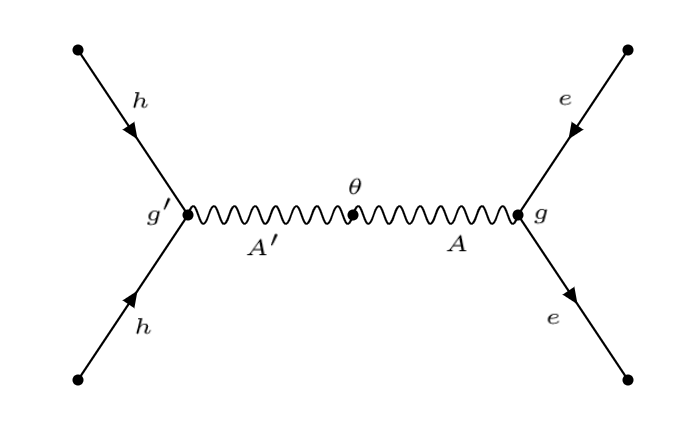
\includegraphics[width=0.8\textwidth]{figures/theory/diagram.png}
\caption{ A Feynman diagram of a dark sector particle $h$ interacting with atomic electrons. $g^{\prime}$ is the gauge coupling to $A^{\prime}$ in the dark sector, $\theta$ the kinetic mixing angle between $A^{\prime}$ and $A$, and $g$ is the usual electromagnetic gauge coupling, $g=e$.  }
\label{fig:diagram}
\end{center}
\end{figure}


\begin{figure}[htbp]
\begin{center}
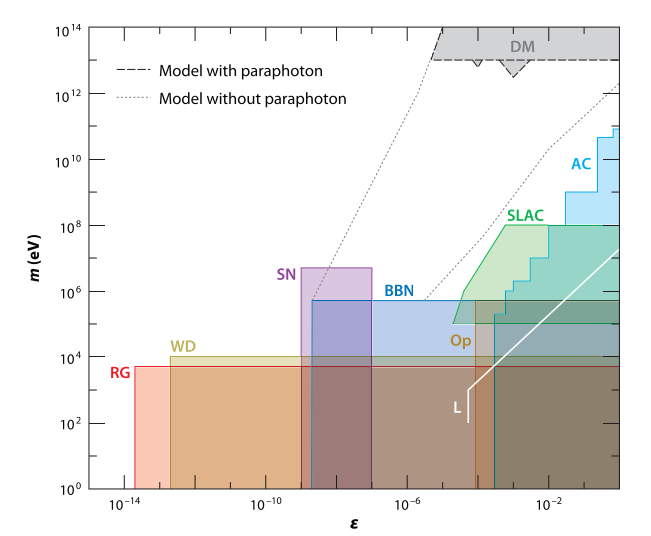
\includegraphics[width=0.8\textwidth]{figures/theory/lip_constraints.png}
\caption{Regions of mass-charge space ruled out for \acs{LIP}s from several different sources. The dashed line limits apply in the case of a dark sector photon (our case of interest), and the dotted line is the limit without dark photons. Abbreviations: AC, accelerator experiments; Op, search for the invisible decay of ortho-positronium; SLAC, the SLAC millicharged particle search; L, the Lamb shift; BBN, big bang nucleosynthesis; RG, plasmon decay in red giants; WD, plasmon decay in white dwarfs; DM, dark matter searches; SN, Supernova 1987A.  Figure from \cite{Perl2009}. }
\label{fig:lip_constraints}
\end{center}
\end{figure}

Unlike many of the constraints in Figure~\ref{fig:lip_constraints}, a search for fractionally charged cosmic rays is model independent. That is, it does not depend on the particular production mechanism of the \ac{LIP}, nor on its mass. A tacit assumption is made that the cosmic ray is high energy, and indeed such high energy \ac{LIP}s may be produced in the present era in violent astrophysical processes or between interaction of ordinary cosmic rays in the atmosphere \cite{Perl2009}. The analysis in Chapter~\ref{ch:lips} concerns the search for \ac{LIP} cosmic rays. The search sensitivity for \ac{LIP} cosmic ray searches is given in terms of flux, $\Phi$, with units cm$^{-2}$~sr$^{-1}$~s$^{-1}$ as a function of the ``charge fraction'' $f$, where $f$ is defined as the denominator of the \ac{LIP} fractional charge, $e/f$. See Figure~\ref{fig:lip_lims} for recent \ac{LIP} flux limits. 

\begin{figure}[htbp]
\begin{center}
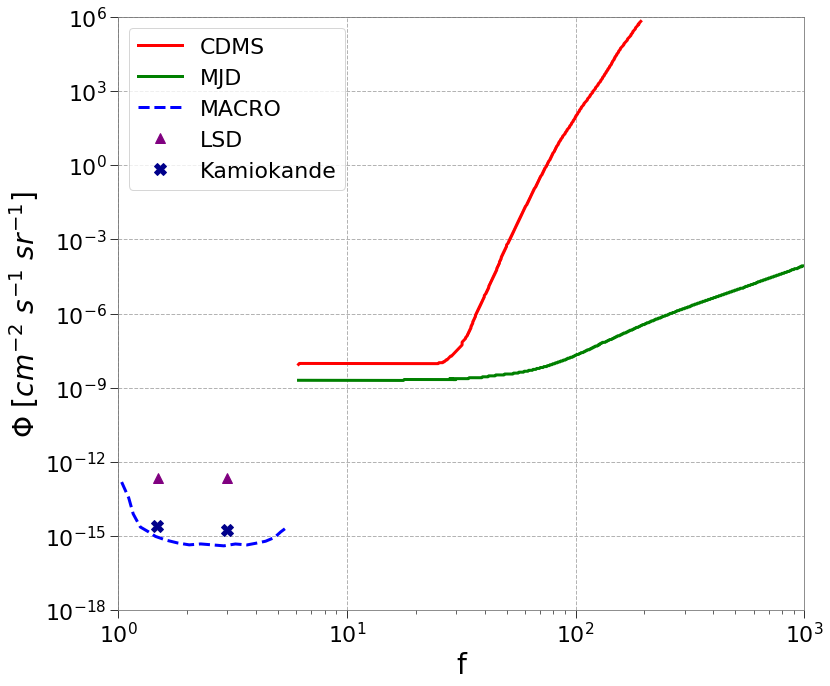
\includegraphics[width=0.8\textwidth]{figures/theory/lip_limits.png}
\caption{Recent limits on the flux of \acs{LIP}s with charge $e/f$ where $f$ is the x-axis. Figure reproduced from \cite{Alvis2018}. }
\label{fig:lip_lims}
\end{center}
\end{figure}


\subsection{WIMPless Miracle and the New Physics Flavor Problem}
As with any dark matter candidate, it is desirable for hidden sector dark matter to have the correct relic density. In Section~\ref{sec:wimp_miracle}, we discussed the \ac{WIMP} miracle: how a particle with a weak scale mass and coupling undergoes thermal freezeout to naturally produce the correct relic abundance. There is a similar situation for the hidden sector dubbed the ``\ac{WIMP}less miracle'', which is much more general. Recall that for a stable thermal relic particle $\chi$, the relic density $\Omega_{\chi}$ goes as:

\begin{equation}
\Omega_{\chi} \sim \langle \sigma_{A}v \rangle^{-1} \sim \frac{m_{\chi}^{2}}{g_{\chi}^{4}}
\end{equation}

The \ac{WIMP} miracle says that for $m_{\chi} \sim m_{weak}$ and $g_{\chi} \sim g_{weak}$, $\Omega_{\chi} \approx \Omega_{cdm}$. For a particle that interacts via a known \ac{SM} force, the weak force is the only reasonable choice, so $g_{\chi} \sim g_{weak}$. Hidden sector dark matter, however, has its own matter content and gauge forces, so many combinations of $(m_{\chi}, g_{\chi})$ are possible. This generalizes the \ac{WIMP} miracle to the \ac{WIMP}less miracle: hidden sector dark matter can produce the correct relic density, but need not have weak scale mass nor interact via the weak force (Figure~\ref{fig:wimpless_miracle}).  
In the case of hidden sector mediated \ac{SUSY} breaking\footnote{\ac{SUSY} is a symmetry that must be broken, otherwise a host of problems would be present. For example, without a broken \ac{SUSY}, the electron and selectron would have the same mass. Furthermore, selectrons are bosons. If we lived in a world where both electrons and selectrons were common, we would not have atomic structure because orbital fermionic electrons are a higher energy state than infinite ground state selectrons.}, it's not merely a coincidence that $(m_{\chi}, g_{\chi})$ can be constrained to a line, but rather that a fixed ratio of $m_{\chi}/g_{\chi}^{2}$ is well-motivated \cite{Feng2008}.

\begin{figure}[htbp]
\begin{center}
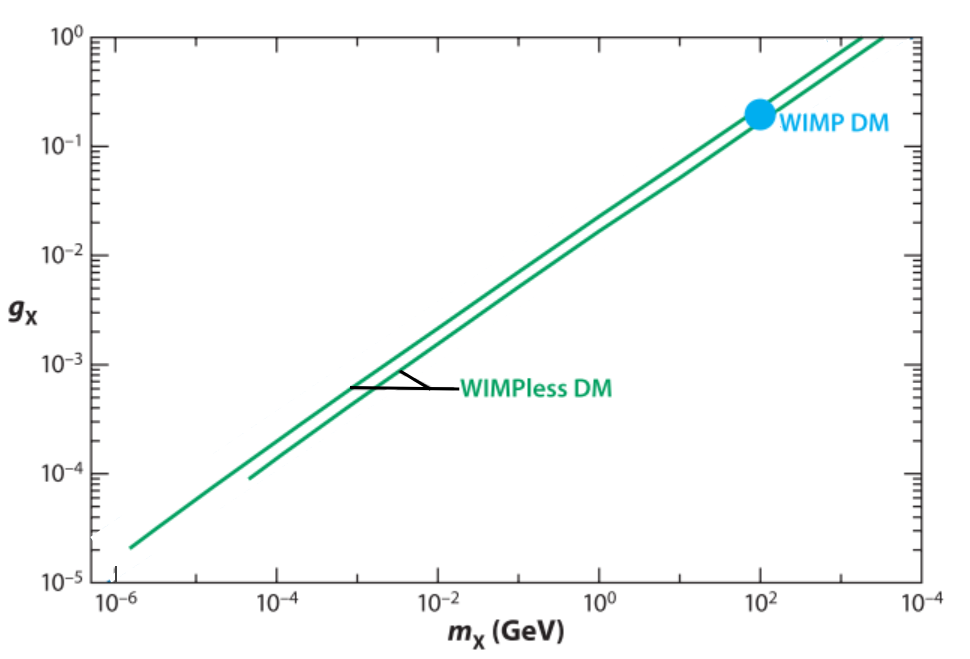
\includegraphics[width=0.8\textwidth]{figures/theory/wimpless_miracle.png}
\caption{Contours in the $(m_{\chi}, g_{\chi})$-plane for two different temperature conditions for the hidden sector. The upper line is for a hidden sector that achieves 80\% of the visible sector temperature after reheating, the lower line is for 30\%. For this plot, the hidden sector in assumed to be a 1-generation flavor-free version of the minimal supersymmetric standard model. Figure adapted from \cite{Feng2010}. }
\label{fig:wimpless_miracle}
\end{center}
\end{figure}

Recall also from Section~\ref{sec:wimp_miracle}, that in addition to it producing the correct relic abundance, the \ac{WIMP} is a favored dark matter candidate because it is related to \ac{SUSY}, which is introduced to solve the hierarchy problem of the \ac{SM}. In attempting to solve the gauge hierarchy problem, \ac{SUSY} gives rise to another problem called the ``new physics flavor problem'' \cite{Feng2010}. \ac{SUSY} particles may violate baryon number, lepton number, flavor, or CP. At the same time, we observe these symmetries to be extremely well preserved in the \ac{SM}. The new physics flavor problem, in a nutshell, is that not all \ac{SUSY} models are capable of elegantly conserving these symmetries. Creating models that solve the new physics flavor problem is a ``prime driver in the field of supersymmetric model building'' \cite{Feng2010}.  A particularly elegant subset of \ac{SUSY} models that do solve the new physics flavor problems are known as \ac{GMSB}. In these models, a hidden sector mediates \ac{SUSY} breaking. In \ac{WIMP}less scenarios, one asks why the hidden sector dark matter should be stable. For \ac{GMSB} models, which solve the new physics flavor problem, an elegant way to stabilize the hidden sector dark matter is through the hidden U(1) charge conservation, which necessitates a massless gauge boson in the hidden sector. This is precisely the situation we have with \ac{LIP}s. To quote \cite{Feng2010}: ``In summary, hidden sector dark matter models may in fact be motivated by leading problems in particle physics, and may even have naturally the correct relic density, through a generalization of the \ac{WIMP} miracle to the \ac{WIMP}less miracle.''

\subsection{Charge Quantization}
It is known experimentally that all charged particles in the \ac{SM} have charge $\pm\frac{1}{3}e$, $\pm\frac{2}{3}e$, or $\pm e$. However, there is no theoretical motivation behind this quantization of electric charge. Holdom suggested a new, U(1) with a ``paraphoton'' gauge boson could produce quantized charge in the \ac{SM} and transfer fractional shifts to fermions that interact with the paraphoton \cite{Holdom1986}, which is the \ac{LIP} paradigm. Others, \cite{Foot1993}, \cite{Babu1990}, \cite{Schellekens1990}, \cite{Wen1985}, and \cite{Dirac1931}, have proposed various extensions to the \ac{SM} that would produce charge quantization. Some of these theories yield fractionally charged particles, and all of them require new physics beyond the \ac{SM}. It is useful to note that even outside of the hidden sector, there are theoretical motivations for fractionally charged particles. 


\section{Experimental Strategies for Detecting Dark Matter}
\label{sec:dm_detection_schemes}
Experiments designed to detect dark matter, be it \ac{WIMP}, axion, dark sector, or other candidates, fall into three main categories: production, indirect detection, and direct detection (see Figure~\ref{fig:dm_detection_schemes}). Detection schemes and examples are discussed in the following subsections. All three methods are in use to provide a diverse, multipronged \ac{DM} detection program. 

\begin{figure}[htbp]
\begin{center}
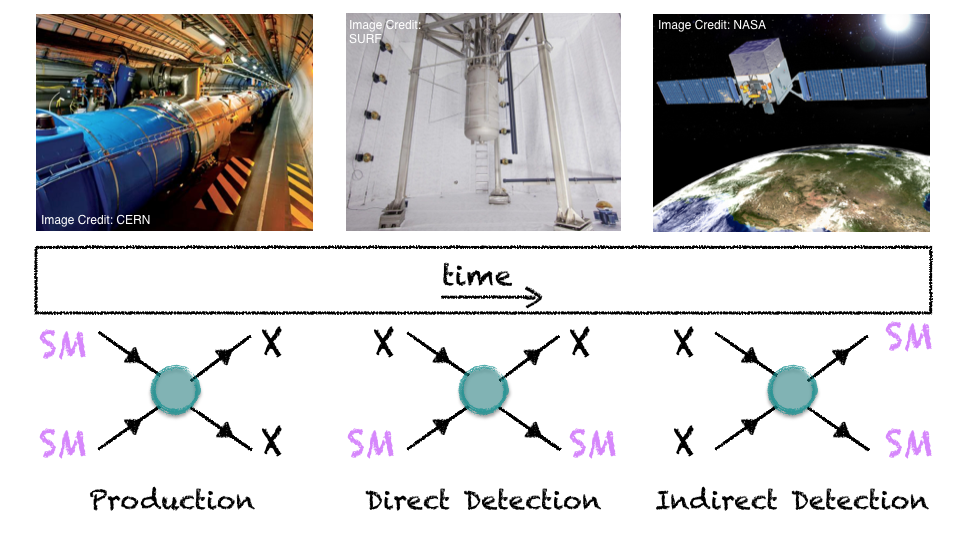
\includegraphics[width=\textwidth]{figures/theory/dm_detection_schemes.png}
\caption{Summary of \acs{DM} detection schemes with illustrative Feynman diagrams. In all cases, the arrow of time is from left to right. (left) \acs{SM} particles can be collided at high energy facilities, which may produce \acs{DM} particles, $\chi$. (center) $\chi$ may scatter with \acs{SM} particles, leaving behind a characteristic signal. (right) $\chi$ particles in the galaxy may annihilate and produce \acs{SM} particles, which produces an \acs{SM} signal in excess of expectations from standard astrophysical processes.}
\label{fig:dm_detection_schemes}
\end{center}
\end{figure}

\subsection{Production}
Colliders like the \ac{LHC} are capable of accelerating \ac{SM} particles to high energies. The \ac{SM} particles, typically protons, antiprotons, electrons, and/or positrons, can be collided with each other or with a fixed target. In general, dark matter produced in these collisions appears as ``missing energy'' when the event is reconstructed. A classic signal of a new, non-interacting particle is missing missing momentum transverse to the beam line, indicating the particle escaped without interacting in the detector. A recent overview of collider searches for several different dark matter candidates can be found in \cite{Penning2018}. 

\subsubsection{LIP Production}
It is noted in \cite{Perl2009} that ``high-energy electron-positron colliders provide the most definitive search method among accelerator and collider searches for fractionally charge particles [in the range $\pm\frac{1}{3}e -\pm \frac{4}{3}e$].'' This is due to the production cross section being large and known to high accuracy. Another successful collider method to search for fractionally charged particles with charge $<<1$ is called a ```beam dump''. In beam dump experiments, the collider accelerates e.g. an electron into a fixed target, producing secondary particles. A large mass of shielding is between the target and the detector. Only secondary particles with a small charge can make it through the shielding to reach the detector. The limit in Figure~\ref{fig:lip_constraints} titled SLAC is from a beam dump type experiment; see \cite{Prinz1998} for details about the SLAC millicharged particle search. Hadron colliders can also look for such particles, albeit with more restrictions \cite{Perl2009}. 

\subsection{Indirect Detection}
The signal of dark matter annihilation can appear in both ground-based and satellite detectors. Dark matter may decay or annihilate into \ac{SM} particles, which can be detected by conventional detectors. Positive identification of an indirect dark matter signal is difficult due to large potential backgrounds from astrophysical sources, which are not perfectly understood. However, indirect detection can probe questions collider and direct searches cannot, such as whether \ac{DM} is perfectly stable and what the annihilation cross sections are. 

\subsubsection{LIP Indirect Detection}
Indirect limits for fractionally charged particles come from stellar evolution and supernovae (see limits titled WD, RG, and SN in Figure~\ref{fig:lip_constraints}). Essentially, new low-mass particles can be produced in the hot and dense medium of stars, and eventually escape, carrying away energy \cite{Davidson2000}. The additional energy-loss channel modifies stellar evolution, and observations of brightness, etc. can set a limit on the \ac{LIP} mass and interaction strength. For Supernova 1987A, the number of neutrinos detected at Earth roughly agrees with theoretical expectations. If fractionally charged particles contribute to cooling, the neutrino flux would decrease; the SN limit in Figure~\ref{fig:lip_constraints} is from such an analysis \cite{Perl2009} \cite{Davidson2000}.

\subsection{Direct Detection}
In direct detection, experimentalists seek to observe \ac{DM} interactions in a detector composed of \ac{SM} materials. Detectors are designed with a \ac{DM} candidate in mind, and aspects of the detector are optimized at the design stage to search for one type of \ac{DM}. Because direct detection searches are built with a particular \ac{DM} candidate in mind, backgrounds can be controlled and minimized much more than in indirect or production searches. Experimental conditions can even be improved by designing for lower backgrounds for the candidate of interest; such changes cannot be applied to indirect searches. Of course, a given detector can search for \ac{DM} candidate even if it was not initially designed/optimized to do so, and in this case, the search still benefits from the detailed understanding of backgrounds in the detector. Most current direct detection experiments fall into one of two categories: \ac{WIMP} detector or axion detector. In the case of \ac{WIMP} detectors, the detector target material is some homogenous material like solid Ge or liquid Xe, and experimentalists seek to detect energy deposition consistent with that of a \ac{WIMP} causing a nuclear recoil in the target. This type of detector must be composed of radiopure materials and located deep underground to be capable of detecting rare \ac{WIMP} interactions. In the case of axions, the detector is a resonator cavity or circut with a strong magnetic field, which couples with the axion field. Cosmic rays and radioactivity are not backgrounds for axion detection, so these detectors need not be placed underground or built of radiopure materials; however, their electronic noise must be strictly managed. Axion detectors take advantage of a resonance amplification of their signal that would occur at a specific axion mass and coupling. To observe the resonance signal, detector background noise must be kept sufficiently low. 

\subsubsection{LIP Direct Detection}
Direct detection searches for fractionally charged particles include schemes like the Millikan drop experiment, which modern methods have improved upon (see \cite{Perl2009} for more detail). Table-top style experiments searching for anomalous decay of ortho-positronium, or changes in the Lamb shift, would indicate additional couplings to a hidden sector \cite{Perl2009}; these are marked Op and L in Figure~\ref{fig:lip_constraints}, respectively. Searches for cosmogenic \ac{LIP}s can also be accomplished by a variety of detectors and detector technologies. These types of searches set limits on the flux \ac{LIP}s as a function of charge fraction. Limits from previous cosmogenic \ac{LIP} searches, each described below, can be found Figure~\ref{fig:lip_lims}.

Kamiokande II, a large water Cherenkov detector, carried out a search for \ac{LIP}s of charge $e/3$ and $2e/3$ \cite{Mori1991}. Kamiokande II had a diverse neutrino science program, and made significant contributions to the current understanding of solar, atmospheric, and supernova neutrinos. The detector was fortuitously operational during Supernova 1987A and observed 11 neutrino events from the supernova \cite{Hirata1988}, garnering a Nobel Prize. The detector consisted of a cylindrical steel tank containing 2400 tons of water viewed by 948 20-inch \ac{PMT}s. This inner detector was surrounded by a 4$\pi$ steradian water veto at least 1.2 m thick, viewed by 123 20-inch \ac{PMT}s. The \ac{LIP} search utilized the number of Cherenkov photons detected to distinguish the fractional charges from the integer charge of the muon.  The number of Cherenkov photons emitted per unit path length and unit wavelength is proportional to $(1/f)^{2}$, where $f$ is the denominator of the fractional charge. The fractional charges were simulated by taking real muon events and multiplying the photon yield by $(1/f)^{2}$. Parameter spaces such as total photoelectron yield versus number of hit \ac{PMT} identified a \ac{LIP} region that was distinct from the muon region, providing a detection efficiency. \ac{PMT} hit maps from the simulations were used to distinguish, by-eye, the \ac{LIP}s from stopped muons and other complicated muon behavior in the detector that could reduce the photon yield. A limit was set on the flux of \ac{LIP}s.

LSD, large scintillator detector, also carried out a search for \ac{LIP}s of charge $e/3$ and $2e/3$  \cite{Aglietta1994}. LSD, also known as the Mont Blanc Neutrino Scintillation Detector, was mainly concerned with detecting low energy neutrinos from cosmic sources.  The LSD detector was composed of a modular array of 72 (1 $\times$ 1 $\times$ 1.5)~m$^{3}$ independent counter tanks arranged in 3 layers, with a total mass of 90~tons of C$_{n}$H$_{2n+2}$ liquid scintillator. Each tank was seen by three \ac{PMT}s in a 3-fold coincidence. To reduce external radioactive backgrounds, the whole detector was shielded by shielded by iron, lead, and borex parafine. For the \ac{LIP} search, the approach was to simulate the expected energy loss of the fractional charges in the detector, which show behavior distinct from a muon. Selection cuts were placed to reject muons and select \ac{LIP}s by comparing, e.g. the energy loss in the upper plane to the energy loss in the middle plane. Some background events from muons remained in the signal region due to the muon only passing though 2 tanks, and an accompanying $\gamma$ triggering the third tank. Signals such as these had energy deposition lower than an muon, and they could mimic a \ac{LIP}. Background events such as the muon with $\gamma$ signature were added to the simulation to assess the expected background rate in the \ac{LIP} signal region.  The number of \ac{LIP} candidates from the real data were then compared to the expected background number, and a limit was set.

MACRO, another large scintillator detector, carried out a search for \ac{LIP}s down to a charge of $e/5$  \cite{Ambrosio2000} \cite{Ambrosio2004}. The main goal of MACRO was to search for magnetic monopoles, but it also made measurements relevant to high energy muon and neutrino astronomy \cite{Ambrosio2002}. The MACRO detector was divided into six modules, each of dimension (12.6 $\times$ 12 $\times$ 9.3)~m$^{3}$; the global dimensions were  (76.5 $\times$ 12 $\times$ 9.3)~m$^{3}$ \cite{Ambrosio2002}. Each module contained a combination of scintillation counters, streamer tubes, and nuclear track detectors for a total mass of $\sim$ 5300~tons (see \cite{Ambrosio2002} for more detail). For the \ac{LIP} search, timing information from the streamer tube modules was used to reconstruct a track. \ac{LIP} candidates were required to have a reconstructed track and pass through the entire detector. Based on the track length, \ac{LIP} candidates were further processed to determine the rate of energy loss in the scintillator. This energy deposition was used to distinguish \ac{LIP}s from muons, as the the energy deposited by a \ac{LIP} scales with $(1/f^{2}$) compared to the muon energy deposition. The trigger efficiency of the modules to low energy events was determined with muons that ``clipped'' individual detectors, and the energy resolution was calibrated with low energy $\gamma$ rays from natural radioactivity. Further data cleaning cuts are made to eliminate tracks that passed too close to the edge of a scintillator counter and those where timing information from the streamer tubes and scintillator modules disagree. Four remaining events were investigated by eye and determined to arise from complicated muon behavior, and a limit was set on the \ac{LIP} flux. 

\ac{CDMS}, a cryogenic germanium and silicon detector, carried out the first search for cosmogenic \ac{LIP}s of charge $\leqslant e/6$ \cite{Agnese2015}. \ac{CDMS} was primarily a \ac{WIMP} dark matter search experiment. The \ac{CDMS} detector was composed of alternating Si and Ge modules arranged in stacks of six modules each (``towers''). For the \ac{LIP} search, the probability distribution of energy deposition of \ac{LIP}s of different charge fraction in each tower module was determined. \ac{LIP} candidates were required to pass though each module in a tower and deposit energy consistent with these probability distributions. Tracks were reconstructed based on the $(x,y)$ positions of the energy depositions in each module, and a good track reconstruction was required. The dominant background was from $\gamma$ scattering, which resulted inconsistent energy depositions and poor tracks. Together, the tracking condition and the energy consistency requirements determined a \ac{LIP} signal region, and simulation determined the efficiency for selecting \ac{LIP} events from gamma events. In the search, all events were found to lie outside the signal region and a limit was set on the \ac{LIP} flux. 

\ac{MJD}, also a cryogenic germanium detector, carried out a search in the charge range $\leqslant e/6$, accessing more \ac{LIP} parameter space than the \ac{CDMS} result \cite{Alvis2018}. \ac{MJD} is primarily a neutrinoless double beta decay experiment, seeking to understand if the neutrino is its own antiparticle. The \ac{MJD} detector is composed to several towers of Ge modules, similar to the \ac{CDMS} detector, but with many more towers. For the \ac{LIP} search, the energy deposition of \ac{LIP}s was simulated in order to assess the detection efficiency. A simple tracking algorithm compared the vectors between pairs of triggered modules; for straight tracks, the vectors all ``point'' to the same direction. The backgrounds such as gammas and electrical noise that fit the energy deposition criteria were eliminated with the tracking algorithm and a limit was set on the \ac{LIP} flux. 

A search for cosmic ray \ac{LIP}s is carried out in Chapter~\ref{ch:lips} with the \ac{LUX} experiment, which is also a canonical \ac{WIMP} detector, but uses \ac{LXe} for its target material. More details about \ac{LXe} as a detector medium are found in Chapter~\ref{ch:LXeTPCs}. Details about the \ac{LUX} detector can be found in Chapter~\ref{ch:lux}.

%Searches for cosmogenic \ac{LIP}s were carried out by Kamiokande II \cite{Mori1991}, MACRO \cite{Ambrosio2000} \cite{Ambrosio2004}, and LSD \cite{Aglietta1994} for a charge range between $1$ and $e/6$. The cryogenic germanium detectors CDMS \cite{Agnese2015} and the Majorana Demonstrator \cite{Alvis2018} carried out searches in the charge range $\leqslant e/6$. 

%Large water or liquid scintillator detectors such as Kamiokande and MACRO performed searches for fractionally charged cosmic rays from $e$ down to $e/6$ (see Figure~\ref{fig:lip_lims}). More recent searches from \ac{CDMS} and \ac{MJD} extend the charge fraction range of these searches down to $\sim e/1000$. These last two searches are both from cryogenic Ge detectors designed with other goals in mind -- \ac{CDMS} is a canonical \ac{WIMP} detector and \ac{MJD} is a neutrinoless double beta decay experiment. 




%*****************************************
%*****************************************
%*****************************************
%*****************************************
%*****************************************
